% Options for packages loaded elsewhere
% Options for packages loaded elsewhere
\PassOptionsToPackage{unicode}{hyperref}
\PassOptionsToPackage{hyphens}{url}
\PassOptionsToPackage{dvipsnames,svgnames,x11names}{xcolor}
%
\documentclass[
  letterpaper,
  DIV=11,
  numbers=noendperiod]{scrartcl}
\usepackage{xcolor}
\usepackage{amsmath,amssymb}
\setcounter{secnumdepth}{5}
\usepackage{iftex}
\ifPDFTeX
  \usepackage[T1]{fontenc}
  \usepackage[utf8]{inputenc}
  \usepackage{textcomp} % provide euro and other symbols
\else % if luatex or xetex
  \usepackage{unicode-math} % this also loads fontspec
  \defaultfontfeatures{Scale=MatchLowercase}
  \defaultfontfeatures[\rmfamily]{Ligatures=TeX,Scale=1}
\fi
\usepackage{lmodern}
\ifPDFTeX\else
  % xetex/luatex font selection
\fi
% Use upquote if available, for straight quotes in verbatim environments
\IfFileExists{upquote.sty}{\usepackage{upquote}}{}
\IfFileExists{microtype.sty}{% use microtype if available
  \usepackage[]{microtype}
  \UseMicrotypeSet[protrusion]{basicmath} % disable protrusion for tt fonts
}{}
\makeatletter
\@ifundefined{KOMAClassName}{% if non-KOMA class
  \IfFileExists{parskip.sty}{%
    \usepackage{parskip}
  }{% else
    \setlength{\parindent}{0pt}
    \setlength{\parskip}{6pt plus 2pt minus 1pt}}
}{% if KOMA class
  \KOMAoptions{parskip=half}}
\makeatother
% Make \paragraph and \subparagraph free-standing
\makeatletter
\ifx\paragraph\undefined\else
  \let\oldparagraph\paragraph
  \renewcommand{\paragraph}{
    \@ifstar
      \xxxParagraphStar
      \xxxParagraphNoStar
  }
  \newcommand{\xxxParagraphStar}[1]{\oldparagraph*{#1}\mbox{}}
  \newcommand{\xxxParagraphNoStar}[1]{\oldparagraph{#1}\mbox{}}
\fi
\ifx\subparagraph\undefined\else
  \let\oldsubparagraph\subparagraph
  \renewcommand{\subparagraph}{
    \@ifstar
      \xxxSubParagraphStar
      \xxxSubParagraphNoStar
  }
  \newcommand{\xxxSubParagraphStar}[1]{\oldsubparagraph*{#1}\mbox{}}
  \newcommand{\xxxSubParagraphNoStar}[1]{\oldsubparagraph{#1}\mbox{}}
\fi
\makeatother


\usepackage{longtable,booktabs,array}
\newcounter{none} % for unnumbered tables
\usepackage{calc} % for calculating minipage widths
% Correct order of tables after \paragraph or \subparagraph
\usepackage{etoolbox}
\makeatletter
\patchcmd\longtable{\par}{\if@noskipsec\mbox{}\fi\par}{}{}
\makeatother
% Allow footnotes in longtable head/foot
\IfFileExists{footnotehyper.sty}{\usepackage{footnotehyper}}{\usepackage{footnote}}
\makesavenoteenv{longtable}
\usepackage{graphicx}
\makeatletter
\newsavebox\pandoc@box
\newcommand*\pandocbounded[1]{% scales image to fit in text height/width
  \sbox\pandoc@box{#1}%
  \Gscale@div\@tempa{\textheight}{\dimexpr\ht\pandoc@box+\dp\pandoc@box\relax}%
  \Gscale@div\@tempb{\linewidth}{\wd\pandoc@box}%
  \ifdim\@tempb\p@<\@tempa\p@\let\@tempa\@tempb\fi% select the smaller of both
  \ifdim\@tempa\p@<\p@\scalebox{\@tempa}{\usebox\pandoc@box}%
  \else\usebox{\pandoc@box}%
  \fi%
}
% Set default figure placement to htbp
\def\fps@figure{htbp}
\makeatother


% definitions for citeproc citations
\NewDocumentCommand\citeproctext{}{}
\NewDocumentCommand\citeproc{mm}{%
  \begingroup\def\citeproctext{#2}\cite{#1}\endgroup}
\makeatletter
 % allow citations to break across lines
 \let\@cite@ofmt\@firstofone
 % avoid brackets around text for \cite:
 \def\@biblabel#1{}
 \def\@cite#1#2{{#1\if@tempswa , #2\fi}}
\makeatother
\newlength{\cslhangindent}
\setlength{\cslhangindent}{1.5em}
\newlength{\csllabelwidth}
\setlength{\csllabelwidth}{3em}
\newenvironment{CSLReferences}[2] % #1 hanging-indent, #2 entry-spacing
 {\begin{list}{}{%
  \setlength{\itemindent}{0pt}
  \setlength{\leftmargin}{0pt}
  \setlength{\parsep}{0pt}
  % turn on hanging indent if param 1 is 1
  \ifodd #1
   \setlength{\leftmargin}{\cslhangindent}
   \setlength{\itemindent}{-1\cslhangindent}
  \fi
  % set entry spacing
  \setlength{\itemsep}{#2\baselineskip}}}
 {\end{list}}
\usepackage{calc}
\newcommand{\CSLBlock}[1]{\hfill\break\parbox[t]{\linewidth}{\strut\ignorespaces#1\strut}}
\newcommand{\CSLLeftMargin}[1]{\parbox[t]{\csllabelwidth}{\strut#1\strut}}
\newcommand{\CSLRightInline}[1]{\parbox[t]{\linewidth - \csllabelwidth}{\strut#1\strut}}
\newcommand{\CSLIndent}[1]{\hspace{\cslhangindent}#1}



\setlength{\emergencystretch}{3em} % prevent overfull lines

\providecommand{\tightlist}{%
  \setlength{\itemsep}{0pt}\setlength{\parskip}{0pt}}



 


\KOMAoption{captions}{tableheading}
\makeatletter
\@ifpackageloaded{float}{}{\usepackage{float}}
\floatstyle{plain}
\@ifundefined{c@chapter}{\newfloat{suppfig}{h}{losuppfig}}{\newfloat{suppfig}{h}{losuppfig}[chapter]}
\floatname{suppfig}{Figure S}
\newcommand*\quartosuppfigref[1]{Figure \hyperref[#1]{S\ref{#1}}}
\@ifpackageloaded{caption}{}{\usepackage{caption}}
\DeclareCaptionLabelFormat{quartosuppfigreflabelformat}{#1#2}
\captionsetup[suppfig]{labelformat=quartosuppfigreflabelformat}
\newcommand*\listofsuppfigs{\listof{suppfig}{List of Supplementary Figures}}
\makeatother
\makeatletter
\@ifpackageloaded{float}{}{\usepackage{float}}
\floatstyle{plain}
\@ifundefined{c@chapter}{\newfloat{supptbl}{h}{losupptbl}}{\newfloat{supptbl}{h}{losupptbl}[chapter]}
\floatname{supptbl}{Table S}
\floatstyle{plaintop}
\restylefloat{supptbl}
\newcommand*\quartosupptblref[1]{Table \hyperref[#1]{S\ref{#1}}}
\@ifpackageloaded{caption}{}{\usepackage{caption}}
\DeclareCaptionLabelFormat{quartosupptblreflabelformat}{#1#2}
\captionsetup[supptbl]{labelformat=quartosupptblreflabelformat}
\newcommand*\listofsupptbls{\listof{supptbl}{List of Supplementary Tables}}
\makeatother
\makeatletter
\@ifpackageloaded{caption}{}{\usepackage{caption}}
\AtBeginDocument{%
\ifdefined\contentsname
  \renewcommand*\contentsname{Table of contents}
\else
  \newcommand\contentsname{Table of contents}
\fi
\ifdefined\listfigurename
  \renewcommand*\listfigurename{List of Figures}
\else
  \newcommand\listfigurename{List of Figures}
\fi
\ifdefined\listtablename
  \renewcommand*\listtablename{List of Tables}
\else
  \newcommand\listtablename{List of Tables}
\fi
\ifdefined\figurename
  \renewcommand*\figurename{Figure}
\else
  \newcommand\figurename{Figure}
\fi
\ifdefined\tablename
  \renewcommand*\tablename{Table}
\else
  \newcommand\tablename{Table}
\fi
}
\@ifpackageloaded{float}{}{\usepackage{float}}
\floatstyle{ruled}
\@ifundefined{c@chapter}{\newfloat{codelisting}{h}{lop}}{\newfloat{codelisting}{h}{lop}[chapter]}
\floatname{codelisting}{Listing}
\newcommand*\listoflistings{\listof{codelisting}{List of Listings}}
\makeatother
\makeatletter
\makeatother
\makeatletter
\@ifpackageloaded{caption}{}{\usepackage{caption}}
\@ifpackageloaded{subcaption}{}{\usepackage{subcaption}}
\makeatother
\usepackage{bookmark}
\IfFileExists{xurl.sty}{\usepackage{xurl}}{} % add URL line breaks if available
\urlstyle{same}
\hypersetup{
  pdftitle={Task-structured preferences guide forward planning in sequential decision-making},
  pdfauthor={Alex Lepauvre; Florian Ott; Stefan Kiebel},
  pdfkeywords={Decision making, Reinforcement learning},
  colorlinks=true,
  linkcolor={blue},
  filecolor={Maroon},
  citecolor={Blue},
  urlcolor={Blue},
  pdfcreator={LaTeX via pandoc}}


\title{Task-structured preferences guide forward planning in sequential
decision-making}
\author{Alex Lepauvre \and Florian Ott \and Stefan Kiebel}
\date{2026-09-18}
\begin{document}
\maketitle
\begin{abstract}
Everyday problems often require choosing among actions with different
future consequences, even though fully evaluating those consequences is
often computationally infeasible. The human brain is remarkable in its
ability to solve such complex problems efficiently. In this paper, we
hypothesize that this capacity arises from a principle inspired by
Bayesian accounts of perception and sensorimotor control: evidence
derived from effortful forward planning is integrated with task-specific
preferences akin to priors, weighted by the uncertainty of these
preferences. To test this hypothesis, we used a sequential
decision-making task with a relatively large state space. Model
comparison showed that participants' deviations from optimal forward
planning are best captured by task-specific preferences, rather than by
unsystematic errors, recent action-history effects, or offer-context
biases. Moreover, the influence of forward planning on participants'
responses depended on preference uncertainty, as evidenced by both
choice behavior and reaction times, and preferences were not arbitrary
but instead supported above-stochastic performance even in the absence
of forward planning. Together, these results are consistent with a
Bayesian-inspired interpretation of decision making, in which costly
forward planning is integrated with state-dependent priors or
preferences. These preferences may provide an inexpensive, quickly
available first-pass solution, which is complemented by forward planning
when preference-based guidance is uncertain.
\end{abstract}


\section{Introduction}\label{introduction}

A central idea in Bayesian accounts of perception and sensorimotor
control is that the brain does not rely on current sensory evidence
alone (Knill and Pouget 2004; Lee and Mumford 2003; Pouget et al. 2013;
Clark 2013; Friston 2010) because sensory evidence is often noisy,
incomplete, or costly to acquire with high precision. Prior information
can reduce this uncertainty by providing an efficient summary of
regularities learned from experience and from the statistical structure
of the environment. Bayesian accounts provide an influential framework
for describing this integration of current evidence and prior
information. In this framework, the influence of prior information
depends on uncertainty: when current evidence is unreliable, behavior
should rely more strongly on the prior. Conversely, when current
evidence is reliable, it should dominate behavior. For example, Körding
and Wolpert (2004) provided a canonical demonstration of this principle,
showing that participants combine learned priors with sensory feedback
according to their relative uncertainty.

A similar logic may apply to decision-making based on forward planning,
where choices require evaluating the future consequences of currently
available actions. Here, we use the term forward planning in a
computational sense: it refers to the estimation of future action
consequences, not necessarily to a consciously accessible process of
deliberation. In this case, evidence consists of estimates of
state-action values internally generated by the computational process
implementing forward planning in the brain, similar to how sensory
organs gather evidence by sampling the environment according to Bayesian
accounts of perception. . In sequential decision tasks, forward planning
can generate such estimates by evaluating the future consequences of
each action in the current state. However, generating these estimates is
typically computationally costly, because it requires evaluating future
outcomes in complex and dynamic environments ({Sutton et al.} 1998;
Gershman et al. 2015; Callaway et al. 2022). In analogy to the Bayesian
view on perception, agents may therefore combine their evidence,
i.e.\,their internal estimates about future consequences, with prior
information about which actions are usually appropriate in a given task.
In this view, action selection reflects a balance between a costly
state-specific estimate and a stored prior tendency to act in a
particular way. This idea has been applied previously in a Bayesian
account of the balance between habitual and goal-directed control, in
which habitual tendencies were modelled as priors over policies that are
balanced against goal-directed information about current outcome
contingencies (Schwöbel et al. 2021, 2024). This approach also resonates
with resource-rational accounts of planning, which postulates that the
brain adapts its planning computations to the costs and benefits of
using its relatively limited cognitive resources (Gershman et al. 2015;
Lai and Gershman 2021; Callaway et al. 2022; Tishby and Polani 2010;
Parush et al. 2011).

This leads to the central hypothesis of the present study: choice
behavior in complex sequential decision-making integrates two sources of
action guidance. First, participants may rely on task-specific
preferences that summarize regularities learned from task structure or
experience. Second, they may use forward planning, as for example
typically modelled by reinforcement learning, to compute state-specific
action values on the current trial. Assuming a Bayesian approach, we
hypothesize that these two sources are integrated by weighting the
contribution of forward planning against preferences by their respective
uncertainties. This hypothesis implies that on trials where uncertainty
about preferences is low, choices should be guided mainly by the
preferences, producing faster responses because less forward planning is
needed. On trials with less certain preferences, decision making should
be more weighted towards forward planning and consequently, response
times should be increased due to the increase in computations.

In this paper, we test this hypothesis in a complex sequential
decision-making task, using choice model comparisons and response-time
analyses. Specifically, we use optimal forward planning as a reference
model and ask whether participants' deviations from this reference are
systematic and better explained by including task-specific preferences.
We compare this account against several alternative models of how
participants may combine planning-derived decision values with potential
preferences. Participants' choices were best captured by a model
combining forward planning with task-specific preferences from multiple
task features. Response-time analyses converged with this pattern,
showing that forward planning conflict slowed responses most when
preferences were weak. Together, these findings suggest that costly
forward planning is integrated with structured, task-informed
preferences that enable faster and less computationally demanding
choices when they provide a clear action tendency.

\section{Results}\label{results}

We tested our hypothesis on a dataset where participants performed a
complex sequential decision making task (Ott et al. (2022b), see
Section~\ref{sec-data-desgin} for the full description of the design).
In each trial, participants had to decide whether to accept or reject an
offer varying between 1 and 4 points, where accepting an offer incurred
and energy cost between 1 and 2 points, and rejecting an offer incurred
a gain of one energy point. Energy cost associated with accepting an
offer changed every 4 trials (referred to as trials segment) and
participants were informed of the current and future trials segment.
This task is highly structure, as each trial consists of a combination
of 4 factors (offer, energy, current and future costs), all of which
have to be taken into account to maximize return, making this dataset
ideal to test our prediction that participants combine forward-planning
with preferences reflecting the structure of the task.

Performance indicates that participants were able to perform the task
well. Participants provided responses with an average reaction time (RT)
of 0.90s \(\pm\) 0.26 (s.d.) and failed to give their response before
time out in only 0.27\% \(\pm\) 0.56 (s.d.) out of 240 trials. On
average, participants gathered 332.43 \(\pm\) 6.64 points throughout the
experiment.

\subsection{Choice behavior}\label{choice-behavior}

To test whether and how participants choice behavior deviates from
optimal planning, we compared four Bayesian hierarchical logistic
regression models of participants accept/reject choices (see
Section~\ref{sec-choice-behavior-modeling-method} for detailed
explanation). All models shared the same planning component: decision
values (DV) obtained by backward induction on the task Markov Decision
Process (MDP), reflecting the difference in long term value between
accepting and rejecting an offer in each state under the optimal policy.
The Planning model contained only DV as a regressor assumed deviations
were unsystematic noise, serving as a benchmark. The three other models
differed in how they accounted for deviations from this benchmark. The
Frequency-prior model assumed deviations reflect a recency bias towards
recently chosen actions. The Offer-context model, the best fitting model
from Ott et al. (2022a), assumed that participants plan to different
extents in extreme versus intermediate offers. Finally, the Preference
model, impelementing our main hypothesis, combined the planning
component with a state-dependent preference score, contructed by
assigning weights to the levels of each task factor (offer, energy,
current and future costs) and summing them, as well as a modulation term
testing whether the influence of planning depends on the entropy of the
preference score.

Model comparison revealed that participants' deviations from optimal
forward planning were indeed systematic. Replicating Ott et al. (2022a),
the Planning model provided the poorest fit
(\(\Delta ELPD_{pref - planning}\)=586.28 \(\pm\) 55.56 s.e., see
Figure~\ref{fig-choicemdl} A), indicating that deviations from optimal
behavior are not purely stochastic. Furthermore, our results indicate
that participants' biases do not reflect a frequency prior
(\(\Delta ELPD_{pref - frequency}\)=581.38 \(\pm\) 55.66), nor a
splitting of the task into separate contexts
(\(\Delta ELPD_{pref - context}\)=165.49 \(\pm\) 52.62). Rather,
participants exhibit preferences that reflect the task structure, as the
Preference model provided the best fit (see Figure~\ref{fig-choicemdl}
A).

This result is highly consistent across participants: the preference
model provided the best fit for 34 out of 40 participants (see
Figure~\ref{fig-choicemdl} B). The improved fit of the preference model
is reflected in Figure~\ref{fig-choicemdl} C, showing the proportion of
correct choice predictions separately for each model and offer values.
Here, the data show that the proportion of matches is on average higher
for the preference compared to all other models.

The estimated factor-level preference weights associated with each task
factor reveal structured biases in participants' behavior (see
Figure~\ref{fig-choicemdl} D and
\quartosupptblref{supptbl-pref_model_param} for the posterior of each
fitted parameter). Participants tend to reject low offers (1 and 2) more
frequently than optimal forward planning would suggest, while they show
a bias towards accepting high offers (3 and 4). These biases are
stronger for extreme offers (1 and 4) compared to intermediate ones (2
and 3). The energy state also plays a critical role in shaping
participants' decisions. When energy is at maximum (e = 6), participants
almost always accept offers, even when rejecting would be more
reward-maximizing. This behavior is intuitive: rejecting offers at max
energy does not yield additional energy, so participants prioritize
immediate rewards, even at the expense of future rewards. In contrast,
when energy is at 0, participants rarely accept offers, even though the
planner predicts a small probability of acceptance
(\textasciitilde0.25). This discrepancy arises because the planner
calculates DV based on long-term returns, where the difference between
accepting and rejecting at energy = 0 is negative but relatively small.
However, participants adopt a stricter rejection policy, likely
reflecting an aversion to accepting offers that yield no immediate
reward. Importantly, energy = 0 occurs in only 17.85\% \(\pm\) 4.02 of
trials, so this counterintuitive effect at energy 0 cannot alone explain
the success of the Preference model. Finally, costs (both current and
future) exert a weaker influence on participants' behavior, with a mild
bias towards accepting offers when costs are low.

\begin{figure}[H]

\centering{

\pandocbounded{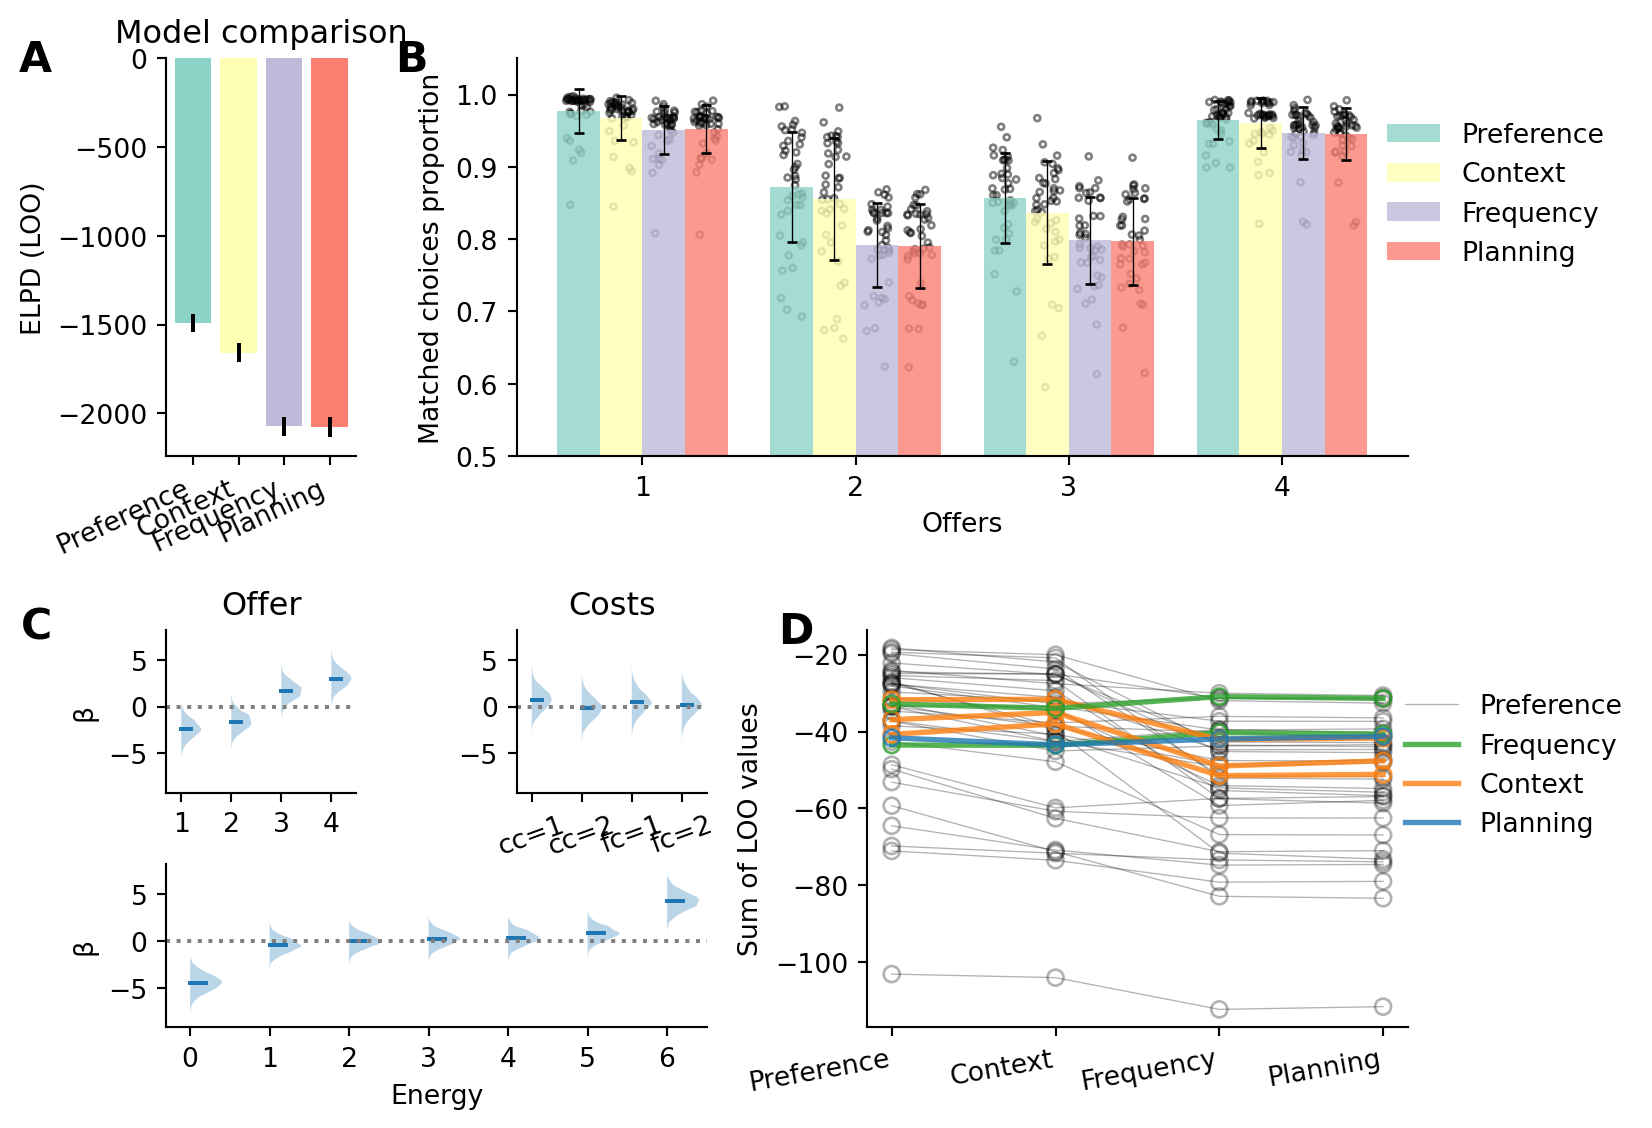
\includegraphics[keepaspectratio]{index_files/figure-pdf/fig-choicemdl-output-1.png}}

}

\caption{\label{fig-choicemdl}Choice-model comparison and fitted
factor-level preference weights (A) Model comparison showing the
expected log pointwise predictive density (ELPD) for each model
(Preference, Offer-context, Frequency-prior and Planning models). Values
closer to 0 indicate better fit. See Table S1 for additional model
comparisons results. (B) Participant-wise best-fitting models. Each
participant is color-coded according to the model with the highest
predictive accuracy. The Preference model provided the best fit for 34
of 40 participants. (C) Observed and model-predicted probability of
accepting, shown separately for each offer level and model. Points
indicate participants' observed acceptance probabilities. (D) Estimated
factor-level preference weights for the Preference model. Panels show
weights for offer levels, current and future cost, and energy levels.
Distributions show the group-level posterior estimates; central bars
indicate medians, and dotted lines indicate the 2.5\% and 97.5\%
quantiles. Dots indicate participant-level mean estimates.}

\end{figure}%

We then proceeded to test the central prediction that the influence of
forward planning should depend on preference uncertainty, quantified as
the entropy of the action tendency implied by the preference score. The
Preference model revealed a positive modulation of forward planning by
preference entropy (\(\beta_{modulation}\)=1.26, \(CI_{95\%}\)={[}0.35,
2.25{]}), indicating that planning-derived DV had a stronger influence
on choices when preferences were more uncertain. Conversely, when
preference had lower entropy, choices were less influenced by
planning-derived DV and were more strongly guided by the preference
score.

This modulation is illustrated in
Figure~\ref{fig-pref-planning-interaction} A, where we plotted the
fitted probability of accepting as a function of planning-derived DV for
different preference scores. Reflecting the main effect of preference
score, the logistic curve shifted leftward as the preference score
increased. Thus, when preference score favored accepting participants
required lower DV to accept an offer. Conversely, when preference score
favored rejecting, higher planning-derived DV were required to overcome
this preference and lead to acceptance. Reflecting the modulation of
preference entropy on DV, the slope of the curve decreases as the
preference score deviates further from zero (in either direction)
reflecting reduced reliance on forward planning as preferences'
uncertainty decreases. Figure~\ref{fig-pref-planning-interaction} B and
C show the observed probability of accepting an offer as a function of
DV, separately when preference scores were positive
(Figure~\ref{fig-pref-planning-interaction} B) and negative
(Figure~\ref{fig-pref-planning-interaction} C). This further shows the
effect of preferences on participants' response choice: participants
accept an offer at lower DV when preference scores are positive than
when preference scores are negative (see
\quartosuppfigref{suppfig-pref-planning-interaction} for unbinned
participants' responses and fitted values as a function of DV and
preference score).

\begin{figure}[H]

\centering{


\includegraphics[width=7.67708in,height=10.09375in]{index_files/figure-pdf/fig-pref-planning-interaction-output-1.png}

}

\caption{\label{fig-pref-planning-interaction}Relationship between
preference score and DV. (A) Fitted probability of accepting an offer as
a function of DV, separately for preference score of {[}-4, -2, -1, 0,
1, 2, 4{]}, to highlight the modulation of preference scores on the
influence of DV. Lines represent the mean of the posterior distribution;
the shaded area is the 95\% C.I. (B) Offer acceptance probability
(y-axis) binned per DV (x-axis), for trials in which preference score is
positive. (C) Same as (B), but for trials in which preference score is
negative. Only bins containing observed trials are shown; the different
number of bars in panels B and C reflects the unequal distribution of
positive- and negative-preference trials across the planning-DV range.
This asymmetry arises because negative preference scores are more often
associated with states in which forward planning also favors rejection.}

\end{figure}%

We next asked whether the fitted forward planning and preference-related
quantities were relevant not only for predicting trial-by-trial choices,
but also for explaining individual differences in overall task
performance. Specifically, we tested whether overall task performance
was related to participants' reliance on forward planning, their
preference entropy, and the extent to which preference uncertainty
modulated forward planning. As larger \(\beta_{plan}\) values indicate
stronger reliance on forward planning, we expected participants with
larger \(\beta_{plan}\) to obtain higher returns. In contrast to forward
planning, preferences might not necessarily maximize reward, so
participants with \,lower preferences entropy should obtain lower return
on average. Finally, larger \(\beta_{modulation}\) indicate that
participants plan more when their preferences are weak
(i.e.\,preferences entropy is larger) and should accordingly obtain
larger returns compared to participants who do not engage more strongly
in forward planning when their preferences are weak. Accordingly, we
predicted that \(\beta_{plan}\), preference entropy and
\(\beta_{modulation}\) should be positively correlated with return.

In line with these predictions, we observed a positive correlation
between \(\beta_{plan}\) and return (r=0.58, p\textless0.001,
Figure~\ref{fig-returns} A), showing that participants who rely more on
forward planning get larger returns. Furthermore, \(\beta_{modulation}\)
is strongly and positively correlated with return (r=0.66,
p\textless0.001, Figure~\ref{fig-returns} C). However, contrary to our
prediction, we observed a negative though only marginally significant
correlation between preference entropy and return (r=-0.29, p=0.072,
Figure~\ref{fig-returns} B). Visual inspection of
Figure~\ref{fig-returns} B revealed that the correlation appears to be
driven from the participant with very low return (2.63 s.d. from
population mean). When removing this participant, the correlation
between preference entropy and return is not marginally significant
(r=-0.09, p=0.596), while it remains strongly significant for forward
planning (r=0.47, p=0.003) and modulation (r=0.60, p\textless0.001) when
the same subject is removed.

\begin{figure}[H]

\centering{

\pandocbounded{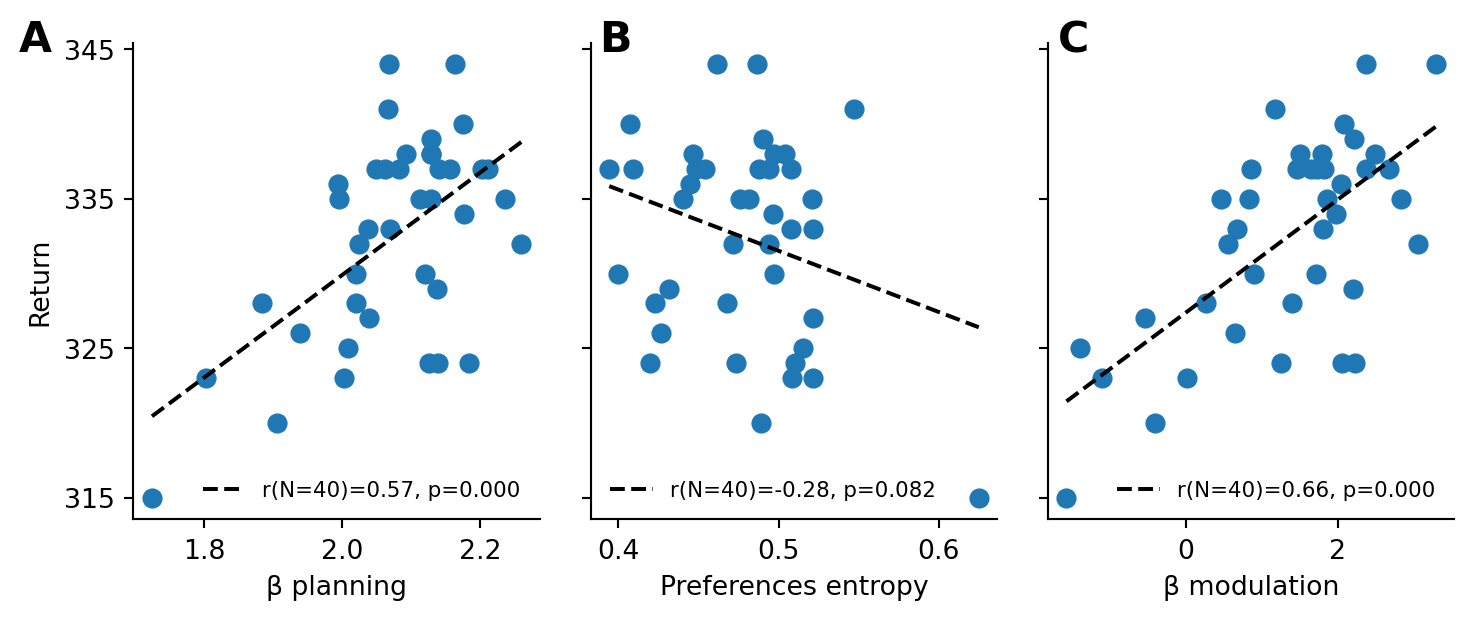
\includegraphics[keepaspectratio]{index_files/figure-pdf/fig-returns-output-1.png}}

}

\caption{\label{fig-returns}Relationship between fitted parameters and
task performance (A) Correlation between participants' total return and
their fitted forward planning sensitivity \(\beta_{plan}\) parameter.
Each dot represents one participant. The line shows an ordinary
least-squares regression fit, where the legend reports Pearson's
correlation and the corresponding p-value. (B) Correlation between
participants' total return and their average preference entropy.
Plotting conventions are the same as in (A). (C) Correlation between
participants' total return and the fitted preference-modulation
parameter \(\beta_{modulation}\). Plotting conventions are the same as
in (A).}

\end{figure}%

\subsection{Experimental factors
relevance}\label{experimental-factors-relevance}

Our results indicate that participants' choices are shaped by two
sources of information: planning-derived values and task-specific
preference scores. These preference scores are not a single global bias.
Instead, under the Preference model, state-dependent preferences reflect
a trial-wise weighted sum of preferences associated with different
factors of the task such as the offer, the current cost context, and
upcoming transitions. Importantly, not all features of the task are
weighted equally. Figure~\ref{fig-choicemdl} C shows that the parameters
associated with offers and energy weigh strongly in participants'
preference scores compared to costs (both current and future). The
fitted factor-level preference weights already suggested that
participants' preference scores were structured primarily by offer value
and energy. We further confirmed this pattern from a complementary
model-comparison perspective. To do so, we compared the full Preference
model with reduced models in which the factor-level preference was
removed for one task factor at a time (see
Section~\ref{sec-factor-relevance-analysis} for a description). This
effectively tests how decision-making changes when participants are
assumed to ignore one specific source of task information, such as offer
value, action costs, or future transitions.

Figure~\ref{fig-task-features} A shows the change in model fit when each
preference factor was removed separately from the full preference model.
Each reduced model omitted the preference term for one experimental
factor while retaining the remaining preference terms. Larger values
indicate that the specific factor is more relevant for the full model's
fit. We found that offer (\(\Delta ELPD_{full - offer}\)=137.36 \(\pm\)
54.44 s.e.), followed by energy (\(\Delta ELPD_{full - energy}\)=133.97
\(\pm\) 51.57 s.e.), has a much larger impact on participants' final
responses, whereas costs-related preferences have a smaller impact on
the overall fit (\(\Delta ELPD_{full - CC}\)=47.02 \(\pm\) 49.89 s.e.
and \(\Delta ELPD_{full - FC}\)=27.35 \(\pm\) 48.62 s.e.).

\begin{figure}[H]

\centering{

\pandocbounded{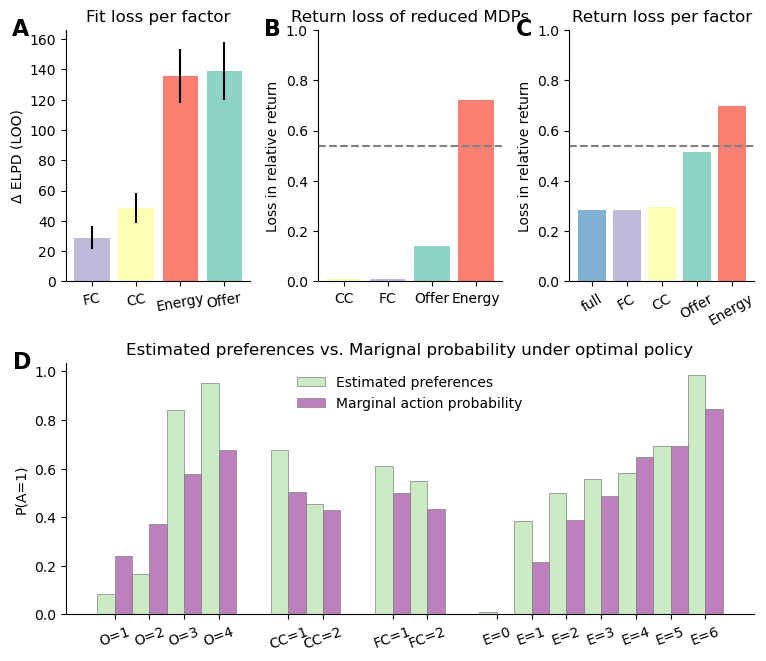
\includegraphics[keepaspectratio]{index_files/figure-pdf/fig-task-features-output-1.png}}

}

\caption{\label{fig-task-features}Contribution of task factors to
preference-based choice and performance. (A) Predictive contribution of
individual preference factors. Difference in fit between the full
Preference model and models in which each of the experimental factors
was removed from preference score estimations in turn. Bars show ΔELPD,
computed as the ELPD of the full model minus the ELPD of the
corresponding reduced model. Values closer to 0 indicate that a factor
does not lead to a strong improvement of the model fit (i.e.\,the factor
weighs less in participants' final decision). (B) Loss in return by
ignoring individual task factors during forward planning (0 indicates no
loss compared to the return under the optimal policy derived from the
full MDP). Bars show the reward sensitivity of each task factor: larger
values indicate that the omitted factor was more important for
reward-maximizing planning. (C) Return loss of policies derived from the
preference score of the full and reduced Preference models, in which the
preference terms for one task factor were omitted in turn. For each
model (full and reduced), we derived a policy from the preference score
alone and calculated the expected return under such a policy, relative
to the optimal policy. The y-axis represents the loss in relative
return; 0 indicates that a preference policy performs exactly as well as
the optimal policy. The horizonal dashed line represents the return
associated with a fully stochastic policy (i.e.\,equal probability of
each action in each state). (D) Per factor-levels accept tendencies in
the fitted preferences and in the optimal policy. For each level of each
task factor, we calculated the accept tendency implied by the fitted
factor-level preference weight and the average accept tendency of the
optimal policy in states containing that feature level, after averaging
over all other task factors. Similar profiles indicate that
participants' preferences capture task regularities present in the
optimal policy; deviations indicate feature-specific biases.}

\end{figure}%

We further sought to determine whether the fitted preferences could
serve as adaptive biases when forward planning is absent. As a first
step, we quantified how strongly optimal return depends on each task
factor. To do so, we derived policies from reduced forward planning
models in which one task factor was ignored and computed their return
loss relative to the optimal policy (Figure~\ref{fig-task-features} B,
see Section~\ref{sec-factor-relevance-analysis}). Our results show that
ignoring current and future costs when planning leads only to minimal
losses (0.78\% and 0.98\% respectively), while ignoring the offer level
leads to a 13.94\% loss. The biggest loss is incurred when ignoring
energy levels. This leads to a loss in returns of 72.04\%, which is even
larger than a purely stochastic policy (i.e., equal probability of
accepting and rejecting an offer on each trial). This indicates that
reward maximization under forward planning is highly sensitive to
energy. This large loss reflects the structure of the task. A policy
that ignores energy cannot adapt choices to the current energy budget.
As a result, it can deplete energy in low-energy states as its behavior
is driven by offer levels. The large reward sensitivity of energy is not
mirrored in Figure~\ref{fig-task-features} A because that analysis
measures the additional predictive contribution of preference terms
after accounting for planning-derived decision-values. Energy is already
strongly reflected by the forward planning component, so removing
energy-related preference terms has a smaller effect on model fit than
its relevance for optimal return would suggest.

Further, we asked whether the fitted preferences could support adaptive
choice when forward planning is absent. If preferences capture useful
task structure, policies derived from the preference score alone should
be suboptimal but still produce less return loss than a stochastic
policy. In addition, removing task factors that strongly shape
participants' preferences should reduce the return of these preference
policies. To quantify this, we computed the expected return loss of
policies derived from the preference score alone (see
Section~\ref{sec-factor-relevance-analysis}). The full preference policy
produced a return loss of 28.34\%, indicating that preferences did not
fully replace forward planning, see Figure~\ref{fig-task-features} C.
However, this loss was smaller than the loss of a stochastic policy
(dashed line), showing that the fitted preferences captured task
structure that was relevant for return maximization
(Figure~\ref{fig-task-features} C). Removing current or future cost from
the preference policy produced little additional loss relative to the
full preference policy (29.72 and 28.38 respectively). In contrast,
removing offer value led to a substantial loss in return of 51.52\%. The
largest loss occurred when energy was removed (69.80\% loss), with
performance falling below that of the stochastic policy. This suggests
that an energy-blind preference policy is not merely less informative
but can become systematically maladaptive by accepting attractive offers
without regard to the current energy budget, making the agent more
likely to run out of energy than under a stochastic policy.

Together, these results suggest that participants' preferences were not
arbitrary biases, but adaptive approximations to optimal choice. They
supported relatively good performance even in the absence of forward
planning (loss of 28.34\% from optimal returns) and provide a useful
first-pass policy that can support good performance when forward
planning is limited but can be further refined by planning-derived DV
when more computation is available.

How do participants derive such adaptive preferences? A potential
explanation is that participants have access to some approximation of
the marginal action probability associated with each factor of the task
under the optimal policy (for example, how often should an offer of 1 be
accepted, across all energy and costs levels). To explore whether this
might be contributing to an underlying mechanism for learning
participants' preferences, we computed the factor-dependent marginal
action probability under the optimal policy.
Figure~\ref{fig-task-features} D plots the factor-level preferences
parameters side-by-side with the marginal action probability, showing
that participants' preferences reflect relatively closely the
factor-level specific marginal action probability of the optimal policy,
with some notable deviations. For offer levels 1 and 2, preferences are
lower than marginal action probability, and higher when for offer levels
3 and 4. Across all other tasks levels, participants' preferences are
larger than marginal action probability (except for energy=4),
suggestive of an optimistic bias (i.e.\,a tendency to accept offers more
often than participants should). This optimistic bias might be afforded
by the gain in energy associated with the tendency to reject low offers.
Nonetheless, the overall similarities between both variables suggest
that these marginal action tendencies may have contributed to the
formation of participants' task structured preferences.

\subsection{Reaction times}\label{reaction-times}

Under the proposed hypothesis, participants' reliance on forward
planning should depend on preference entropy. Low preferences entropy
should reduce the need for forward planning and therefore lead to faster
responses, whereas high preferences entropy should increase reliance on
forward planning and thereby lead to slower responses. Previous studies
have shown that RT is positively correlated with forward planning
conflict, indicating that less forward planning is required when the
value associated with each action is more clearly distinct (Ott et al.
2022a; Gluth et al. 2012; Lee and Daunizeau 2021). We therefore expected
preference scores to attenuate the effect of forward planning conflict
on RT: when participants' preferences provide a clear action tendency,
forward planning conflict should have a weaker influence on response
times. To test this prediction, we modelled participants RT using the
absolute decision value (referred to as decision conflict), as well as
the preference score estimated from the choice behavior model, and the
interaction between the two (see Section~\ref{sec-RT-model-method} for a
description of the model).

Indeed, we found that participants' RT was influenced by (i) forward
planning conflict (\(\beta_{conflict}\)=0.11, \(CI_{95\%}\)={[}0.08,
0.13{]}), (ii) preference entropy (\(\beta_{pref}\)=0.45,
\(CI_{95\%}\)={[}0.37, 0.46{]}) and (iii) the modulation effect between
the two (\(\beta_{modulation}\)=0.11, \(CI_{95\%}\)={[}0.06, 0.13{]},
see Figure~\ref{fig-rt} A). This result extends previous findings
showing that participants do not rely on forward planning to the same
extent across all states of the task. Our results suggest that rather
than splitting the task in independent contexts and engaging in forward
planning to a different extent across those {[}ott2022forward{]}, the
differential amount of forward planning across states instead reflects
the fact that participants engage in forward planning more when
preferences are weak. Specifically, as can be seen in
Figure~\ref{fig-rt} B, forward planning depends less on forward planning
conflict when preferences entropy is low (blue line), but more so when
preferences entropy is larger (orange and green lines).

Indeed, we found that participants' RT was influenced by (i) conflict
(\(\beta_{conflict}\)=0.11, \(CI_{95\%}\)={[}0.08, 0.13{]}), (ii)
entropy of preference score (\(\beta_{pref}\)=0.45,
\(CI_{95\%}\)={[}0.37, 0.46{]}) and (iii) the modulatory effect between
the two (\(\beta_{modulation}\)=0.11, \(CI_{95\%}\)={[}0.06, 0.13{]},
see Figure~\ref{fig-rt} A). This result extends on previous findings
showing that participants do not rely on planning to the same extent
across all states of the task. Our results suggest that rather than
splitting the task in independent contexts and engaging in planning to a
different extent across those (Ott et al. 2022a), the differential
amount of planning across states instead reflects the fact that
participants engage in planning more when preferences are weak. The
positive modulatory effect (see Figure~\ref{fig-rt} A) between conflict
and entropy of preferences indicates that the reliance on planning is
modulated by the strength of participants' preferences. Specifically, as
can be seen in Figure~\ref{fig-rt} B, planning depends less on conflict
when preferences are strong (blue line), but more so when preferences
are weaker (orange and green lines).

Together, these response-time results converge with the choice-model
findings. Participants were slowest when planning-derived DV were in
conflict, and task-specific preferences had high entropy, indicating
stronger reliance on forward planning under preference uncertainty
(green line). Conversely, when preferences provided a clear action
tendency, forward planning conflict had a weaker effect on response
times (blue line), suggesting reduced reliance on planning-derived
values.

\begin{figure}[H]

\centering{

\pandocbounded{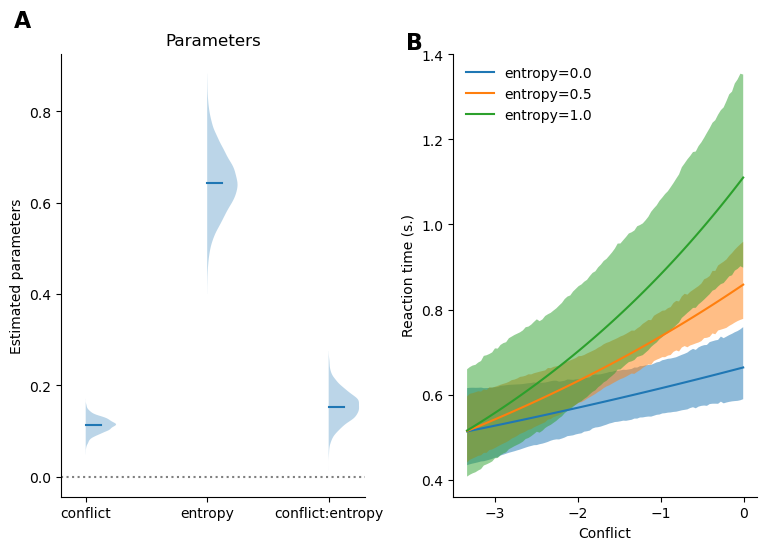
\includegraphics[keepaspectratio]{index_files/figure-pdf/fig-rt-output-2.png}}

}

\caption{\label{fig-rt}RT evidence for preference-modulated forward
planning. (A) Posterior distributions of the fitted response-time
effects, including forward planning conflict, preference entropy, and
their interaction. (B) Posterior predictive curves depicting the
predicted RT as a function of forward planning conflict, separately for
preference entropy of 0, 0.5 and 1.0.}

\end{figure}%

\section{Discussion}\label{discussion}

We found that participants' deviations from an optimal forward planning
reference were systematically organized by task-specific preferences,
and that these preferences regulated the influence of planning-derived
decision values on choice. This pattern was not well explained by
unsystematic errors, recent action-history effects, or the offer-context
biases identified in previous work. Instead, participants' choices were
best explained by a model that combined planning-derived decision values
with task-specific preferences over offers, energy, and costs.
Crucially, these preferences did not act only as additive choice biases.
Planning-derived values had the strongest influence on choice when
preference uncertainty was high, whereas lower preference uncertainty
was associated with reduced planning-related computation, as evidenced
by participants' RT. Additional policy analyses indicated that these
preferences preserved reward-relevant task structure and supported
substantially higher returns than stochastic choice even without forward
planning, although they remained below the optimal forward planning
policy. Feature-wise analyses showed that these preferences captured
reward-relevant structures of the task. Together, these results suggest
that participants used task-specific preferences as efficient
approximations to reward-maximizing choice, while relying more strongly
on forward planning when these preferences did not provide a clear
action tendency.

This finding reframes task-factor effects in sequential decision-making.
Rather than treating offer, energy, and cost effects as separate
descriptive biases, the present account interprets them as structured
action tendencies that interact with planning-derived values.
Computational models of sequential decision-making often include
additional parameters capturing response biases, perseveration, or other
deviations from value-based choice (Ott et al. 2022a, 2020; Ho et al.
2022; Huys et al. 2012; Schwartenbeck et al. 2015). However, these terms
are typically low-dimensional and are not usually decomposed according
to the structure of the task. Conversely, factorial analyses of
experimental data can quantify how different task factors influence
behavior or neural responses (Barr et al. 2013; Baayen and Milin 2010;
{Ashburner et al.} 2014; Singmann and Kellen 2019), but they do not by
themselves specify how these effects relate to forward planning. By
combining these approaches, our model treats task-factor effects as
structured action tendencies that can guide choices and modulate
reliance on planning-derived values.

Our approach was motivated by Bayesian accounts of perception and
sensorimotor control, in which current evidence is integrated with prior
information according to their relative uncertainty Körding and Wolpert
(2004). An intuitive interpretation of our results is that task-specific
preferences play the role of priors, whereas planning-derived values
provide the likelihood-like, state-specific evidence about which action
will lead to better future outcomes, and the entropy of the priors
determines the extent of forward planning. In our task, this
interpretation is particularly evident in how preferences guide behavior
in different states. In states where the relevant features jointly imply
a clear action tendency (e.g.\,high offer, low cost and high energy),
preferences alone may be sufficient to support efficient
decision-making, requiring minimal forward planning. In other states,
different features support opposing actions. For instance, a moderate
offer may favor rejection, whereas low cost and high energy may favor
acceptance. Such opposing factor-level tendencies produce a preference
score closer to zero and therefore higher preference uncertainty. In
such cases, forward planning can help resolve the remaining ambiguity by
evaluating the future consequences of the available actions.

Our model resembles the policy compression framework, under which
forward planning values are integrated with action priors in a Bayesian
fashion (Lai and Gershman 2021). Importantly, this framework assumes
state-independent priors, reflecting the marginal action probability
under the current policy(Lai and Gershman 2021). While such priors work
well with small state spaces or tasks with limited downstream
consequences (Lai and Gershman 2024; Bari and Gershman 2023; Liu and
Gershman 2025; Lai et al. 2022; Gershman and Lak 2025), they may be
insufficient in more complex, sequential decision-making tasks, where
action--state combinations have complex downstream implications. Our
results suggest that participants rely on state-dependent preferences in
such tasks. The factorized preference components strike a balance
between fully state-specific priors, which would be overly costly in
terms of memory and completely state-independent action priors that
would be too coarse-grained to be useful in complex tasks.

Together, these findings provide a potential refinement of the
context-dependent planning effects reported by Ott et al. (2022a). In
that study, participants showed a greater propensity to engage in
forward planning for intermediate offers (2 and 3) than for extreme
offers (1 and 4), with model comparisons supporting a coarse partition
of the state space into these offer contexts. Our results suggest a more
general principle: intermediate offers are associated with less decisive
preference-based action tendencies, and therefore with greater reliance
on planning-derived values. Thus, rather than varying only across
predefined offer contexts, planning-related control may vary with
preference uncertainty over the relevant task factors, including offer,
energy, current cost, and future cost.

Our results contribute to the debate about whether deviations from
optimality reflect systematic errors or adaptive heuristics. Across
psychology and perceptual decision-making, deviations from normative
models have often been described as systematic errors (Tversky and
Kahneman 1974; Gilovich and Griffin 2002; Rahnev and Denison 2018;
Berthet and De Gardelle 2023). In contrast, biases can also be
interpreted as adaptive heuristics that provide computationally
inexpensive shortcuts and support effective, though not necessarily
optimal, solutions in complex tasks ({Gigerenzer et al.} 2000; Tsetsos
et al. 2016; Gigerenzer and Brighton 2009). In line with an
adaptive-heuristic interpretation, our findings suggest that preferences
were not arbitrary residuals around an optimal-planning process. Rather,
they appeared to capture structured action tendencies derived from task
features, which supported above-stochastic performance even in the
absence of forward planning. Deviations from optimal forward planning
may partly reflect inexpensive, task-specific action tendencies that
provide a useful first-pass guide, while being complemented by forward
planning when further evaluation is needed. This pattern suggests that
preference-based guidance and planning-derived evaluation interact
within a single decision process, rather than reflecting a simple
opposition between heuristic bias and optimal forward planning.

Importantly, while the Preference model suggests that task-specific
preferences can function like prior action tendencies, the model is
rather descriptive in the sense that it does not establish that the
fitted preferences are priors in a formal Bayesian sense. In addition,
the model implies that the preferences were stable during the modelled
task phase and does not capture updating of these preferences. The
similarity between preferences and factor levels-dependent marginal
action probabilities (see Figure~\ref{fig-task-features} D) suggests
that preferences might arise by keeping track of actions performed at
each level of each factor under an approximately optimal policy. For
example, this may have happened in the initial training session (Ruge
and Wolfensteller 2010). Furthermore, general schemas from encounters
with similar naturally occurring problems in the environment (budgeting
decisions in everyday life), or explicit instructions highlighting
relevant features might also play a role in fast learning of
preferences. A key question for future research is whether such
preferences function as state-dependent action priors, and how agents
determine the task features that are relevant for constructing and
learning these priors, especially in real-world settings where task
structure is not always explicit.

While our model uses backward induction to derive state-action values,
this does not imply that the brain implements forward planning in this
way. Biologically plausible forward planning may rely on approximate
algorithms such as sampling, partial tree search and approximate value
computations ({Sutton et al.} 1998; {Silver et al.} 2016; Huys et al.
2012; Schwöbel et al. 2021). We are not committed to any one of these
alternatives, as our main interest in the paper was to investigate the
structure underlying participants' deviations from forward planning. The
observed interaction between RT, preferences entropy and forward
planning conflict suggests that whichever algorithm implements action
value estimation in the brain, the extent of planning-related
computation can be adaptively adjusted to obtain estimates of different
precision, depending on preferences entropy. Developing RL or active
inference agents equipped with such structured priors and testing their
predictions against human data may be important for understanding the
emergence and utility of efficient, adaptive decision strategies in
complex environments.

The present account makes several testable predictions about when
preference-based guidance should dominate. Reliance on preferences
should increase when task features provide a clear action tendency, when
forward planning time is limited, or when the marginal value of
additional computation is low. Conversely, reliance on forward planning
should increase when task features provide conflicting action
tendencies, when future consequences are difficult to infer from local
features alone, or when the cost of an error is high. Future experiments
could test these predictions by manipulating factors such as time
pressure, training, instructions, and task familiarity, planning
horizon, task volatility, or the reliability of feature-based cues. Such
manipulations could help disentangle the sources of task-specific
preferences and clarify how structured priors are formed, adapted and
integrated with forward planning.

\section{Methods}\label{methods}

\subsection{Data}\label{sec-data-desgin}

The data used in this study were published by Ott and colleagues
(2022a). In this study, \texttt{\{python\}\ f"\{n\_participants:.0f\}"}
participants
(\texttt{\{python\}\ f"\{n\_female:.0f\},\ mean\ age=\{mean\_age:.1f\},\ SD=\{std\_age:.1f\}"})
took part in a sequential decision-making task (Ott et al. 2022a,
2022b). The study was approved by the Institutional Review Board of the
Technische Universität Dresden and conducted in accordance with ethical
standards of the Declaration of Helsinki.

Figure~\ref{fig-design} shows a schematic representation of the task.
Participants were instructed to gather as many points as possible
throughout the task. In each trial, they were presented with an offer
associated with a reward of either 1, 2, 3 or 4 points, which they could
either accept or reject. To accept the offer in a trial, participants
had to pay an energy cost of either 1 or 2 energy points (low cost, LC
and high cost, HC respectively). When they rejected the offer, they
gained 1 energy point. Participants' energy level was capped at 6, so
their energy could range from 0 (depleted energy) to 6 (max energy).
Offers varied in each trial following a uniform distribution. Costs
remained fixed for 4 consecutive trials, which we refer to as a segment
(see Figure~\ref{fig-design} B), and participants were informed of the
price of the current segment and the next segment. The cost of the next
segment was pseudorandomized to equate the probability of each
transition (from current HC or LC to future HC or LC, see
Figure~\ref{fig-design} C) and ensure that each transition occurred 15
times. When participants accepted an offer that they could not afford
(current energy level below current cost), no reward was awarded and a
warning was displayed.

\begin{figure}

\centering{

\pandocbounded{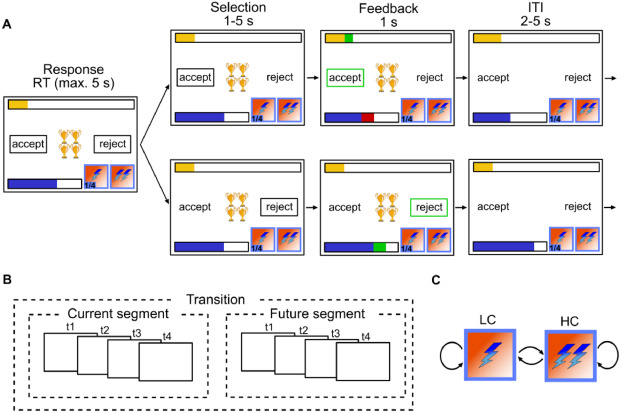
\includegraphics[keepaspectratio,alt={Experimental design}]{images/experimental_design.jpg}}

}

\caption{\label{fig-design}EExperimental design: (A) Single trial
procedure, each frame represents a step within the trial with duration
of each step above. Top row depicts participants accepting; bottom row
depicts participants rejecting. In each trial, participants are
presented with N golden cups; the number of cups symbolizes the amount
of reward. The blue bar represents energy level; yellow bar represents
accumulated reward so far, lightning symbols at the bottom right of each
frame represent current cost (left) and future cost (right). (B) Between
trial costs dependencies. A segment consists of 4 trials and the cost in
each segment is fixed. Participants are aware of the cost in the current
and future 4 trials but not beyond. (C) Transition structure. Cost can
transition from low cost (LC) to high cost (HC), LC to LC, HC to LC and
HC to HC. Reproduced from Ott et al. (2022a)}

\end{figure}%

Accordingly, each trial was defined by several task factors: the current
offer, the participant's current energy level, the current cost of
accepting, and the cost in the upcoming segment. Participants had to
decide whether to accept or reject the offer under the specific
combination of these factors. Because accepting uses up energy while
rejecting replenished it, each choice also changed the state in which
the participant entered subsequent trials. Maximizing overall return was
therefore non-trivial and required considering the future consequences
of current choices.

At the start of each trial, a fixation cross was presented for 0.5 s in
the middle of the screen. Then, an offer appeared represented by the
number of ``cups'' presented in the middle of the screen, and choice
options were presented on each side of the screen, surrounded by a black
frame. Participants had 5 s to provide an answer, by selecting either
option (accept or reject), in which case the frame around the chosen
option disappeared. Following their choice, the resulting change in
energy and points was displayed (green indicating an increase in point
and/or energy, red indicating a decrease in energy) for 1s. The trial
ended with an inter-trial interval (ITI) ranging from 2 to 5 s
(uniformly sampled, rounded to the first decimal) in which the offer
disappeared, and unframed choice options remained on screen. If
participants took longer than 5 s to provide their answer, a warning
message was displayed and the next trial started.

Following their choice, the resulting change in energy and points was
displayed (green indicating an increase in point and/or energy, red
indicating a decrease in energy) for 1s. The trial ended with an
inter-trial interval (ITI) ranging from 2 to 5 s (uniformly sampled,
rounded to the first decimal) in which the offer disappeared, and
unframed choice options remained on screen. If participants took longer
than 5 s to provide their answer, a warning message was displayed and
the next trial started.

To familiarize themselves with the task, participants conducted a
training session of 144 trials, corresponding to 36 segments.
Participants then completed 240 trials (60 segments) which are included
in subsequent analyses. Participants started with an energy budget of 3,
and their reward points were accumulated throughout the entire
experiment. The trials sequence was pseudorandomized, such that each
costs transitions (LC to LC, LC to HC, HC to LC and HC to HC, see
Figure\,1 C) occurred equally often within the training and test
sessions, resulting in 9 repetitions of each transition in the training
session and 15 in the experiment. In addition, the offer sequence was
selected such that the frequency of each offer was matched across costs
transitions. The sequence of costs' transitions and offers was kept the
same across participants. Participants were offered two to three minutes
breaks every 20 segments. The test sessions lasted around 40 min.

\subsection{Forward planning
component}\label{sec-forward_planning_component}

To model optimal behavior in the task, we operationalized our task as a
Markov Decision Process (MDP) with the following tuples:

\[
MDP = (S, A, P, R)
\]

Where \(S\) represents all possible states in our task, where each state
\(s\) consists of a combination of the experimental variables in our
task: \(S=E \times O \times CC \times FC \times T\), with energy
\(E={0, 1, ..., 6}\), offer \(O={1, 2, 3, 4}\), current segment cost
\(CC={1, 2}\), future segment cost \(FC={1, 2}\) and trial
\(T={1, 2,..., 13}\). Time steps (i.e.~trials) had to be incorporated in
the state space to account for the cost being trial dependent. \(A\) is
the set of possible actions in our task (\(accept=1, reject=0\)), \(P\)
is the transitional probability from a given state to all other states
(\(P=P_{\forall s \in S}(s'|s, a)\)), and \(R\) is the reward function
characterizing the reward participants can obtain in a given state for
each action (\(R=R_{\forall s \in S}(s|a)\)).

While optimal behavior would require considering outcomes up until the
end of the task, we modelled forward planning over a limited horizon,
following the approach used by Ott et al. (2022a). Participants had
explicit information about the current and upcoming segment,
corresponding to an eight-trial horizon. Solving the MDP only over these
eight trials would implicitly treat the task as ending after the
upcoming segment, leading the optimal policy to spend all remaining
energy by the end of that horizon. To avoid this terminal artefact, we
included one additional segment beyond the known horizon. Thus, action
values were computed over a twelve-trial planning horizon, with a
terminal value set after the twelfth trial, yielding 13 time points in
the dynamic-programming solution. In the first 8 trials, the probability
of the next state reflects the offer-related stochasticity, while costs
are known. For trials beyond the known horizon, the uncertainty
associated with the offer is compounded by the uncertainty related to
the next cost transition (see Ott et al. 2022a for more details).

We applied backward induction to compute the long-term value associated
with each action in any given state (i.e.~the \(Q\) function {Sutton et
al.} 1998). Participants maximizing return should choose the action with
the largest value. As there were only two possible actions in our task
(accept or reject), we computed decision values (DV) as:

\[
DV_s = Q(s, a=1) - Q(s, a=0)
\]

In states where the DV are negative, participants should reject, and in
states where DV are positive, participants should accept the offer.

\subsection{Modelling of participants
responses}\label{sec-choice-behavior-modeling-method}

Participants responses were modelled using a logistic regression:

\begin{equation}\protect\phantomsection\label{eq-logistic_reg}{
P(a=1) = \sigma(\eta)
}\end{equation}

where \(\sigma(x)=\frac{1}{1+e^-x}\) denotes the logistic sigmoid.

Participants' responses were modelled using Bayesian hierarchical
logistic regressions that estimate the probability of accepting the
current offer. We compared four models that differed in which sources of
information were allowed to influence this probability. All models
included planning-derived DV as a benchmark estimate of optimal action
value. The models differed in how they accounted for systematic
deviations from this forward planning benchmark: as unstructured noise,
recent action frequencies, the Offer-context structure identified in the
original analysis by Ott et al. (2022a), or task-specific preferences.
This comparison builds on previous work by including the best-fitting
model among the 21 models tested by ott2022forward as a strong reference
model. We then asked whether a factorized preference account could
explain participants' choices better than this previous account.
Additional parametrizations, reduced models, and robustness checks are
described in the model-comparison section below and reported in the
supplementary material. Formally, these differences were implemented by
changing the predictors included in the linear predictor \(\eta\). We
describe the models in turn, starting with the planning model and then
adding increasingly structured accounts of participants' deviations from
optimal forward planning.

\subsubsection{Planning model}\label{planning-model}

To establish a benchmark, we first asked whether participants' choices
could be explained by optimal forward planning alone. In this pure
Planning model, participants' responses were modelled only as a function
of the planning-derived DV:

\begin{equation}\protect\phantomsection\label{eq-planning-model}{
\begin{aligned}
\eta_{planning} &= \beta_{plan} \times DV
\end{aligned}
}\end{equation}

This model captures the possibility that participants' deviations from
optimal forward planning are unsystematic. Under this account,
alternative models with additional regressors should not yield better
predictive accuracy once model complexity is taken into account. Any
improvement of the subsequent models would therefore indicate that
deviations from the forward planning benchmark contain systematic
structure.

\subsubsection{Frequency-prior model}\label{frequency-prior-model}

Alternatively, participants' deviations from optimality might reflect a
recency bias, whereby choice on a given trial is biased towards the most
frequent action in recent history. Recent accounts of forward planning
consider that priors consist of a state independent recency bias
(Schwöbel et al. 2021, 2024; Kuperwajs and Ma 2021). Similarly, under
the policy compression framework, the optimal policy integrates forward
planning and marginal action probability across states (Lai and Gershman
2021, 2024). To test whether in our task participants' responses are
biased towards most frequent action taken in previous trials, and
approximate the policy compression framework, we fitted a
Frequency-prior model, which models participants' responses as a
function of DV combined with a recency bias:

\begin{equation}\protect\phantomsection\label{eq-frequency-model}{
\begin{aligned}
\eta_{frequency} =& \beta_{plan} \times DV + \beta_{prior} \times P(A)
\end{aligned}
}\end{equation}

We computed \(P(A)_t\) in each trial \(t\) using a linearly decaying
moving average going back \(k=20\) trials, assuming temporally
discounted effects of past actions (see
\quartosuppfigref{suppfig-frequency_model_comparison} for exploration of
the fit at different \(k\)):

\begin{equation}\protect\phantomsection\label{eq-mvavg}{
\begin{aligned}
P(A)_t =& \frac{\sum_{i=t-k}^{t-1}x_i \times w_i}{\sum_{i=t-k}^{t-1}w_i}
\end{aligned}
}\end{equation}

Where \(x_i\) denotes the action taken on trial i coded as accept or
reject, and \(w=[1, 2, ..., k]\) so that the weights increase linearly
from 1 for the oldest included trial to \(k\) for the most recent trial.

\subsubsection{Offer-context model}\label{offer-context-model}

In addition, we used the best-fitting model (among 21 models) from Ott
et al. (2022a), to test whether participants treat states clusters as
separate contexts in which they plan to different extents. We refer to
this model as the Offer-context model. Here, the forward planning
component (DV) is split between extreme and intermediate offers (offers
{[}1, 4{]} and {[}2, 3{]} respectively) to reflect the fact that
participants treat those as separate contexts, with different control
requirements. In addition, the model comprises offer specific and energy
related flexible biases regressors:

\begin{equation}\protect\phantomsection\label{eq-context-model}{
\begin{aligned}
\eta_{context} =& \beta_{plan23} \times DV_{23} + \beta_{plan14} \times DV_{14} + \\
&\beta_{O1}\mathbf{I}_{O1} + \beta_{O2}\mathbf{I}_{O2} + \beta_{O3}\mathbf{I}_{O3} + \beta_{O4}\mathbf{I}_{O4} + \\
&\beta_{basic}\mathbf{I}_{basic} + \beta_{maxE}\mathbf{I}_{maxE} + \\
&\beta_{minE_{LC}}\mathbf{I}_{minE_{LC}} + \beta_{minE_{HC}}\mathbf{I}_{minE_{HC}} 
\end{aligned}
}\end{equation}

\(\mathbf{I}\) indicate dummy regressors encoding specific experimental
conditions: \(\mathbf{I}_{basic}\) encodes trials where energy is
sufficient to accept the offer and inferior to 6, \(\mathbf{I}_{maxE}\)
encodes trials where energy is equal to 6, \(\mathbf{I}_{minE_{LC}}\)
for trials where energy is too low to accept the offer when cost is low,
\(\mathbf{I}_{minE_{HC}}\) for trials where energy is too low to accept
the offer when cost is high, \(\mathbf{I}_{O1-4}\) for trials with offer
1-4 where energy is sufficient to accept. Following Ott et al. (2022a),
these regressors meant to account for edge cases within the state space
were not included in the Frequency-prior model as it was aimed to test
whether participants' biases from optimal behavior can be uniquely
explained by a frequency bias. These were also not included in the
preference model below, as these regressors consist of a linear
combination of the preference factors of the model and would therefore
be redundant.

\subsubsection{Preferences model}\label{preferences-model}

Finally, we developed a task-specific preference model (Preference model
for short) to test whether participants' choices reflect the integration
of forward planning with task-specific preferences. The model contains
three components. First, as in all other models, choices depend on the
planning-derived DV. Second, choices depend on a state-dependent,
task-specific preference score. This preference score is constructed by
assigning preference weights to the levels of the main task factors
namely offer, energy, current cost, and future cost. We refer to these
as factor-level preferences (i.e., the preference weight associated with
a given level of a given factor). The score is then computed as the sum
of the corresponding factor-level preferences for the current state.
Third, the model includes a modulation term that tests whether the
influence of forward planning depends on the uncertainty of the
preference score. We quantified this uncertainty as the entropy of the
preference score (preference entropy). The model therefore tests the
prediction that participants rely more on forward planning when their
preferences are weak or uncertain:

\begin{equation}\protect\phantomsection\label{eq-preference_model}{
\begin{aligned}
\eta_{pref} &= \beta_{plan} \times DV + pref + \beta_{modulation} \times(H(pref) \times DV)
\end{aligned}
}\end{equation}

Where: \[
\begin{aligned}
pref = \mathbf{X_{pref}}\mathbf{\beta}
\end{aligned}
\]

And \(H(pref)\) is the entropy of the preference score:

\begin{equation}\protect\phantomsection\label{eq-entropy}{
\begin{aligned}
H(pref) = -\sigma(pref) * log(\sigma(pref)) - (1-\sigma(pref)) * log(1-\sigma(pref))
\end{aligned}
}\end{equation}

With:

\begin{equation}\protect\phantomsection\label{eq-entropy}{
\begin{aligned}
\sigma(x) = \frac{1}{1+e^{-x}}
\end{aligned}
}\end{equation}

Participants' factor-level preferences are estimated as latent
variables. \(\mathbf{X_{pref}}\) is a \([M \times N]\) (M=measurements,
N=experimental levels) matrix dummy coding each factor of the
experimental setup (energy, offer, current and future costs) and
\(\mathbf{\beta}\) is a vector of weights estimated for each level of
each factor.

\subsection{Model fitting and
comparison}\label{model-fitting-and-comparison}

Models were fitted to participants' response data using Bayesian
hierarchical logistic regressions implemented using PYMC ({Abril-Pla et
al.} 2023) and Bambi (Capretto et al. 2022). We excluded trials where
participants did not provide a response or if RT exceeded the response
window (5 s). Across models, the following parameters were modelled
hierarchically, with separate participant-level estimates drawn from
group-level distributions:
\(\beta_{plan},\ \beta_{plan23},\ \beta_{plan14},\ \beta_{pref},\ \beta_{modulation},\ \beta_{basic},\ \beta_{O1},\ \beta_{O1},\ \beta_{O2},\ \beta_{O3},\ \beta_{O4}\),
while the remaining parameters were fixed across participants. For all
parameters, we used weakly informative hyperprior distributions
\(\mu \sim \mathcal{N}(0, 2)\) and \(\sigma \sim Halfnormal(0, 2)\). All
models were fitted using 4 chains of 2000 samples each (1000 warmups),
resulting in 4000 samples in total. We report the mean of the posterior
and the 95\% credible interval for the estimated parameters in the text.

We used Pareto-smoothed importance sampling to approximate leave-one-out
cross-validation (PSIS-LOO, Vehtari et al. 2017) to estimate the
expected log pointwise predictive density (ELPD) which we used to
compare the fit of these different models accounting for model
complexity. Furthermore, we performed model comparison within each
single subject to estimate the robustness of the best-fitting model in
our population sample, by computing the sum of the pointwise predictive
accuracy for each participant and model, yielding a score for each
participant and model.

Note that each of the four main models was compared against alternative
parameterizations to ensure the robustness of our findings and rule out
alternative explanations. For example, the Frequency-prior model was
tested with varying temporal integration windows (see
\quartosuppfigref{suppfig-frequency_model_comparison} and
\quartosupptblref{supptbl-frequency_model_comparison}), and the
Offer-context model was selected from a previous study (Ott et al.
2022a) after comparison with 21 alternatives. Similarly, reduced
versions of the Preference model were tested against the full model by
removing each component (forward planning, preference and modulation) as
well as individual task factors (or a total of 7 alternative prefernece
models,see \quartosuppfigref{suppfig-preference_model_comparison} and
\quartosupptblref{supptbl-preferences_model_comparison}). For clarity,
we focus on the four best-fitting models (Planning, Frequency prior,
Offer-context, and Preference models) in the main text, with comparisons
to all alternatives detailed in the supplementary material.

\subsection{Experimental factors relevance
analysis}\label{sec-factor-relevance-analysis}

The Preference model estimates factor-level preference weights for each
task factor (energy, offer, current and future costs), revealing that
participants' deviations from optimal forward planning are more strongly
driven by some factors of the task (energy and offers) than others
(current and future costs). To quantify the behavioral contribution of
each factor, we compared the full preference model to reduced models in
which all factor-level preference regressors from one task factor were
removed. A large decrease in predictive accuracy after removing a factor
indicates that preferences associated with this factor explain a
substantial part of participants' choices beyond the planning-derived
values.

The observation that participants' deviation from optimal forward
planning is systematically influenced by specific task factors raises
the question of whether preferences constitute unhelpful biases
(suboptimal tendencies without adaptive value in the task) or whether
they reflect a structured yet simplified solution to the task. In other
words, could participants' preferences constitute a low-dimensional
decomposition of an approximation of the optimal policy, providing a
cheap alternative to guide behavior in the absence of forward planning?
To test this hypothesis, we conducted a series of analyses to test
whether weights of the factors in participants' preferences relate to
the structure of the task.

First, we asked whether the factors that are strongly weighted in
participants' preference scores are more relevant for reward
maximization. For this purpose, we constructed reduced versions of the
full MDP described in Section~\ref{sec-forward_planning_component},
where one task factor (such as offer, energy\ldots) was omitted by
averaging transition probabilities and rewards across the levels of that
factor. For each reduced MDP, we computed the state action value
function (\(Q_{reduced}\)) and mapped it back onto the full MDP by
assigning the aggregated states' values to their corresponding original
states. Using this mapping, we derived a policy from the reduced MDP and
calculated its expected return in the full MDP. This analysis measures
the reward sensitivity of each task factor: if ignoring a factor leads
to a large loss in return, optimal behavior depends strongly on
information about that factor.

Second, we asked whether participants' preferences themselves define a
useful policy in the absence of forward planning. We derived policies
from the preference score of the full Preference model and from reduced
Preference models in which one task factor was omitted. We then computed
the expected return of each preference-based policy relative to the
optimal policy. If task-specific preferences provide an adaptive
approximation to optimal choice, the full preference policy should
outperform a stochastic policy and removing behaviorally important
factors should reduce expected return.

Finally, we explored a possible source of these preferences. Within the
policy-compression framework, compressed policies can be described in
terms of marginal action probabilities (Lai and Gershman 2021). We
therefore computed, under the optimal policy, the probability of
accepting under each level of each task factor after marginalizing over
all other factors. For example, we computed the frequency with which an
offer of 1 should be accepted across all energy and cost states. We then
compared these factor-specific marginal action probabilities with the
fitted preference weights. A close correspondence would suggest that
participants' preferences may approximate feature-specific marginal
action tendencies of the optimal policy.

\subsection{Reaction times analysis}\label{sec-RT-model-method}

In our task, exact computation of optimal policy is prohibitively
expensive, given the size of the task's state space (1,456 states), the
forward planning horizon, and the highly probabilistic nature of the
task. Preferences derived from task knowledge or from task experience
are presumably readily available to the participants or require minimal
computation. A part of our hypothesis is that instead of systematically
evaluating all future outcomes before making a choice, participants
consider the entropy of their preferences to determine how much they
should engage in forward planning. If so, we would expect participants'
RT to reflect the entropy of their preferences, as more certain
preferences should be associated with less forward planning, resulting
in faster RT.

Ott et al. (2022a) showed that response times were slower when the
planning-derived DV for accepting and rejecting were similar, and that
this forward planning conflict effect was greater for intermediate than
for extreme offers. We reinterpret this context dependence as a
consequence of preference entropy. Intermediate offers tend to generate
weaker preference signals, whereas extreme offers tend to produce
clearer action tendencies. Accordingly, we expected forward planning
conflict to slow responses most when preferences were weak.

To test whether the effect of forward planning conflict should depend on
preference entropy, we modelled participants' RTs as a function of
forward planning conflict (i.e.~\(conflict = - |DV|\)), preference
entropy (fitted in the Preference model) and the modulation of forward
planning by preference entropy:

\begin{equation}\protect\phantomsection\label{eq-RT-model}{
log(RT) = \beta_{conflict} * Conflict + \beta_{pref} * H(pref) + \beta_{modulation} * (Conflict : H(pref))
}\end{equation}

We predicted a positive modulation, such that forward planning conflict
would be associated with longer RTs when preference entropy was high,
that is, when preferences were weak or uncertain.

\section{Acknowledgements}\label{acknowledgements}

\section{Contribution statement}\label{contribution-statement}

Conceptualization: A.L., F.O., S.K.; Data curation: A.L., F.O.; Formal
analysis: A.L.; Funding acquisition: F.O., S.K.; Investigation: A.L.;
Methodology: A.L., S.K.; Project management: A.L.; Resources: S.K.;
Software: A.L.; Supervision: S.K.; Validation: A.L.; Visualization:
A.L., S.K.; Writing - original draft: A.L., S.K.; Writing - review \&
editing: A.L., F.O., S.K.

\section{Data and code statement}\label{data-and-code-statement}

All data used in this paper were previously published as part of Ott et
al. (2022a), and are available at https://zenodo.org/records/6328296.
Code can be found on github
https://github.com/AlexLepauvre/state\_abstraction\_paper. In addition,
we've created a custom toolbox to implement reinforcement learning
algorithm, which can be found here:
https://github.com/AlexLepauvre/state-abstraction

\section{References}\label{references}

\protect\phantomsection\label{refs}
\begin{CSLReferences}{1}{1}
\bibitem[\citeproctext]{ref-abril2023pymc}
{Abril-Pla, Oriol, Virgile Andreani, Colin Carroll, et al.} 2023.
{``PyMC: A Modern, and Comprehensive Probabilistic Programming Framework
in Python.''} \emph{PeerJ Computer Science} 9: e1516.

\bibitem[\citeproctext]{ref-ashburner2014spm12}
{Ashburner, John, Gareth Barnes, Chun-Chuan Chen, et al.} 2014. {``SPM12
Manual.''} \emph{Wellcome Trust Centre for Neuroimaging, London, UK}
2464 (4): 53.

\bibitem[\citeproctext]{ref-baayen2010analyzing}
Baayen, R Harald, and Petar Milin. 2010. {``Analyzing Reaction Times.''}
\emph{International Journal of Psychological Research} 3 (2): 12--28.

\bibitem[\citeproctext]{ref-bari2023undermatching}
Bari, Bilal A, and Samuel J Gershman. 2023. {``Undermatching Is a
Consequence of Policy Compression.''} \emph{Journal of Neuroscience} 43
(3): 447--57.

\bibitem[\citeproctext]{ref-barr2013random}
Barr, Dale J, Roger Levy, Christoph Scheepers, and Harry J Tily. 2013.
{``Random Effects Structure for Confirmatory Hypothesis Testing: Keep It
Maximal.''} \emph{Journal of Memory and Language} 68 (3): 255--78.

\bibitem[\citeproctext]{ref-berthet2023heuristics}
Berthet, Vincent, and Vincent De Gardelle. 2023. {``The
Heuristics-and-Biases Inventory: An Open-Source Tool to Explore
Individual Differences in Rationality.''} \emph{Frontiers in Psychology}
14: 1145246.

\bibitem[\citeproctext]{ref-callaway2022rational}
Callaway, Frederick, Bas Van Opheusden, Sayan Gul, et al. 2022.
{``Rational Use of Cognitive Resources in Human Planning.''}
\emph{Nature Human Behaviour} 6 (8): 1112--25.

\bibitem[\citeproctext]{ref-Capretto2022}
Capretto, Tomás, Camen Piho, Ravin Kumar, Jacob Westfall, Tal Yarkoni,
and Osvaldo A Martin. 2022. {``Bambi: A Simple Interface for Fitting
Bayesian Linear Models in Python.''} \emph{Journal of Statistical
Software} 103 (15): 1--29. \url{https://doi.org/10.18637/jss.v103.i15}.

\bibitem[\citeproctext]{ref-clark2013whatever}
Clark, Andy. 2013. {``Whatever Next? Predictive Brains, Situated Agents,
and the Future of Cognitive Science.''} \emph{Behavioral and Brain
Sciences} 36 (3): 181--204.

\bibitem[\citeproctext]{ref-friston2010free}
Friston, Karl. 2010. {``The Free-Energy Principle: A Unified Brain
Theory?''} \emph{Nature Reviews Neuroscience} 11 (2): 127--38.

\bibitem[\citeproctext]{ref-gershman2015computational}
Gershman, Samuel J, Eric J Horvitz, and Joshua B Tenenbaum. 2015.
{``Computational Rationality: A Converging Paradigm for Intelligence in
Brains, Minds, and Machines.''} \emph{Science} 349 (6245): 273--78.

\bibitem[\citeproctext]{ref-gershman2025policy}
Gershman, Samuel J, and Armin Lak. 2025. {``Policy Complexity Suppresses
Dopamine Responses.''} \emph{Journal of Neuroscience} 45 (9).

\bibitem[\citeproctext]{ref-gigerenzer2009homo}
Gigerenzer, Gerd, and Henry Brighton. 2009. {``Homo Heuristicus: Why
Biased Minds Make Better Inferences.''} \emph{Topics in Cognitive
Science} 1 (1): 107--43.

\bibitem[\citeproctext]{ref-gigerenzer2000simple}
{Gigerenzer, Gerd, Peter M Todd, the ABC Research Group, et al.} 2000.
\emph{Simple Heuristics That Make Us Smart}. Oxford University Press.

\bibitem[\citeproctext]{ref-gilovich2002heuristics}
Gilovich, Thomas, and Dale W Griffin. 2002. \emph{Heuristics and Biases:
The Psychology of Intuitive Judgment}. Cambridge university press.

\bibitem[\citeproctext]{ref-gluth2012deciding}
Gluth, Sebastian, Jörg Rieskamp, and Christian Büchel. 2012. {``Deciding
When to Decide: Time-Variant Sequential Sampling Models Explain the
Emergence of Value-Based Decisions in the Human Brain.''} \emph{Journal
of Neuroscience} 32 (31): 10686--98.

\bibitem[\citeproctext]{ref-ho2022people}
Ho, Mark K, David Abel, Carlos G Correa, Michael L Littman, Jonathan D
Cohen, and Thomas L Griffiths. 2022. {``People Construct Simplified
Mental Representations to Plan.''} \emph{Nature} 606 (7912): 129--36.

\bibitem[\citeproctext]{ref-huys2012bonsai}
Huys, Quentin JM, Neir Eshel, Elizabeth O'Nions, Luke Sheridan, Peter
Dayan, and Jonathan P Roiser. 2012. {``Bonsai Trees in Your Head: How
the Pavlovian System Sculpts Goal-Directed Choices by Pruning Decision
Trees.''} \emph{PLoS Computational Biology} 8 (3): e1002410.

\bibitem[\citeproctext]{ref-knill2004bayesian}
Knill, David C, and Alexandre Pouget. 2004. {``The Bayesian Brain: The
Role of Uncertainty in Neural Coding and Computation.''} \emph{TRENDS in
Neurosciences} 27 (12): 712--19.

\bibitem[\citeproctext]{ref-kording2004bayesian}
Körding, Konrad P, and Daniel M Wolpert. 2004. {``Bayesian Integration
in Sensorimotor Learning.''} \emph{Nature} 427 (6971): 244--47.

\bibitem[\citeproctext]{ref-kuperwajs2021planning}
Kuperwajs, Ionatan, and Wei Ji Ma. 2021. {``Planning to Plan: A Bayesian
Model for Optimizing the Depth of Decision Tree Search.''}
\emph{Proceedings of the Annual Meeting of the Cognitive Science
Society} 43.

\bibitem[\citeproctext]{ref-lai2021policy}
Lai, Lucy, and Samuel J Gershman. 2021. {``Policy Compression: An
Information Bottleneck in Action Selection.''} In \emph{Psychology of
Learning and Motivation}, vol. 74. Elsevier.

\bibitem[\citeproctext]{ref-lai2024human}
Lai, Lucy, and Samuel J Gershman. 2024. {``Human Decision Making
Balances Reward Maximization and Policy Compression.''} \emph{PLOS
Computational Biology} 20 (4): e1012057.

\bibitem[\citeproctext]{ref-lai2022action}
Lai, Lucy, Ann Zixiang Huang, and Samuel J Gershman. 2022. {``Action
Chunking as Policy Compression.''} \emph{PsyArXiv}.

\bibitem[\citeproctext]{ref-lee2021trading}
Lee, Douglas G, and Jean Daunizeau. 2021. {``Trading Mental Effort for
Confidence in the Metacognitive Control of Value-Based
Decision-Making.''} \emph{Elife} 10: e63282.

\bibitem[\citeproctext]{ref-lee2003hierarchical}
Lee, Tai Sing, and David Mumford. 2003. {``Hierarchical Bayesian
Inference in the Visual Cortex.''} \emph{Journal of the Optical Society
of America A} 20 (7): 1434--48.

\bibitem[\citeproctext]{ref-liu2025action}
Liu, Shuze, and Samuel Joseph Gershman. 2025. {``Action Subsampling
Supports Policy Compression in Large Action Spaces.''} \emph{PLOS
Computational Biology} 21 (9): e1013444.

\bibitem[\citeproctext]{ref-ott2022forward}
Ott, Florian, Eric Legler, and Stefan J Kiebel. 2022a. {``Forward
Planning Driven by Context-Dependant Conflict Processing in Anterior
Cingulate Cortex.''} \emph{NeuroImage} 256: 119222.
\url{https://doi.org/10.1016/j.neuroimage.2022.119222}.

\bibitem[\citeproctext]{ref-ott2022forward-data}
Ott, Florian, Eric Legler, and Stefan J Kiebel. 2022b. \emph{Forward
Planning Driven by Context-Dependent Conflict Processing in Anterior
Cingulate Cortex - Analysis Code and Datasets}. V. 1.2. Zenodo,
released. \url{https://doi.org/10.5281/zenodo.6328296}.

\bibitem[\citeproctext]{ref-ott2020dynamic}
Ott, Florian, Dimitrije Marković, Alexander Strobel, and Stefan J
Kiebel. 2020. {``Dynamic Integration of Forward Planning and Heuristic
Preferences During Multiple Goal Pursuit.''} \emph{PLoS Computational
Biology} 16 (2): e1007685.

\bibitem[\citeproctext]{ref-parush2011dopaminergic}
Parush, Naama, Naftali Tishby, and Hagai Bergman. 2011. {``Dopaminergic
Balance Between Reward Maximization and Policy Complexity.''}
\emph{Frontiers in Systems Neuroscience} 5: 22.

\bibitem[\citeproctext]{ref-pouget2013probabilistic}
Pouget, Alexandre, Jeffrey M Beck, Wei Ji Ma, and Peter E Latham. 2013.
{``Probabilistic Brains: Knowns and Unknowns.''} \emph{Nature
Neuroscience} 16 (9): 1170--78.

\bibitem[\citeproctext]{ref-rahnev2018suboptimality}
Rahnev, Dobromir, and Rachel N Denison. 2018. {``Suboptimality in
Perceptual Decision Making.''} \emph{Behavioral and Brain Sciences} 41:
e223.

\bibitem[\citeproctext]{ref-rao1999predictive}
Rao, Rajesh PN, and Dana H Ballard. 1999. {``Predictive Coding in the
Visual Cortex: A Functional Interpretation of Some Extra-Classical
Receptive-Field Effects.''} \emph{Nature Neuroscience} 2 (1): 79--87.

\bibitem[\citeproctext]{ref-ruge2010rapid}
Ruge, Hannes, and Uta Wolfensteller. 2010. {``Rapid Formation of
Pragmatic Rule Representations in the Human Brain During
Instruction-Based Learning.''} \emph{Cerebral Cortex} 20 (7): 1656--67.

\bibitem[\citeproctext]{ref-schwartenbeck2015dopaminergic}
Schwartenbeck, Philipp, Thomas HB FitzGerald, Christoph Mathys, Ray
Dolan, and Karl Friston. 2015. {``The Dopaminergic Midbrain Encodes the
Expected Certainty about Desired Outcomes.''} \emph{Cerebral Cortex} 25
(10): 3434--45.

\bibitem[\citeproctext]{ref-schwobel2024joint}
Schwöbel, Sarah, Dimitrije Marković, Michael N Smolka, and Stefan
Kiebel. 2024. {``Joint Modeling of Choices and Reaction Times Based on
Bayesian Contextual Behavioral Control.''} \emph{PLoS Computational
Biology} 20 (7): e1012228.

\bibitem[\citeproctext]{ref-schwobel2021balancing}
Schwöbel, Sarah, Dimitrije Marković, Michael N Smolka, and Stefan J
Kiebel. 2021. {``Balancing Control: A Bayesian Interpretation of
Habitual and Goal-Directed Behavior.''} \emph{Journal of Mathematical
Psychology} 100: 102472.

\bibitem[\citeproctext]{ref-silver2016mastering}
{Silver, David, Aja Huang, Chris J Maddison, et al.} 2016. {``Mastering
the Game of Go with Deep Neural Networks and Tree Search.''}
\emph{Nature} 529 (7587): 484--89.

\bibitem[\citeproctext]{ref-singmann2019introduction}
Singmann, Henrik, and David Kellen. 2019. {``An Introduction to Mixed
Models for Experimental Psychology.''} In \emph{New Methods in Cognitive
Psychology}. Routledge.

\bibitem[\citeproctext]{ref-sutton1998reinforcement}
{Sutton, Richard S, Andrew G Barto, et al.} 1998. \emph{Reinforcement
Learning: An Introduction}. Vol. 1. MIT press Cambridge.

\bibitem[\citeproctext]{ref-tishby2010information}
Tishby, Naftali, and Daniel Polani. 2010. {``Information Theory of
Decisions and Actions.''} In \emph{Perception-Action Cycle: Models,
Architectures, and Hardware}. Springer.

\bibitem[\citeproctext]{ref-tsetsos2016economic}
Tsetsos, Konstantinos, Rani Moran, James Moreland, Nick Chater, Marius
Usher, and Christopher Summerfield. 2016. {``Economic Irrationality Is
Optimal During Noisy Decision Making.''} \emph{Proceedings of the
National Academy of Sciences} 113 (11): 3102--7.

\bibitem[\citeproctext]{ref-tversky1974judgment}
Tversky, Amos, and Daniel Kahneman. 1974. {``Judgment Under Uncertainty:
Heuristics and Biases: Biases in Judgments Reveal Some Heuristics of
Thinking Under Uncertainty.''} \emph{Science} 185 (4157): 1124--31.

\bibitem[\citeproctext]{ref-vehtari2017practical}
Vehtari, Aki, Andrew Gelman, and Jonah Gabry. 2017. {``Practical
Bayesian Model Evaluation Using Leave-One-Out Cross-Validation and
WAIC.''} \emph{Statistics and Computing} 27 (5): 1413--32.

\end{CSLReferences}

\section{Supplementary material}\label{supplementary-material}

\subsection{Supplementary figures:}\label{supplementary-figures}

\begin{suppfig}

\centering{

\pandocbounded{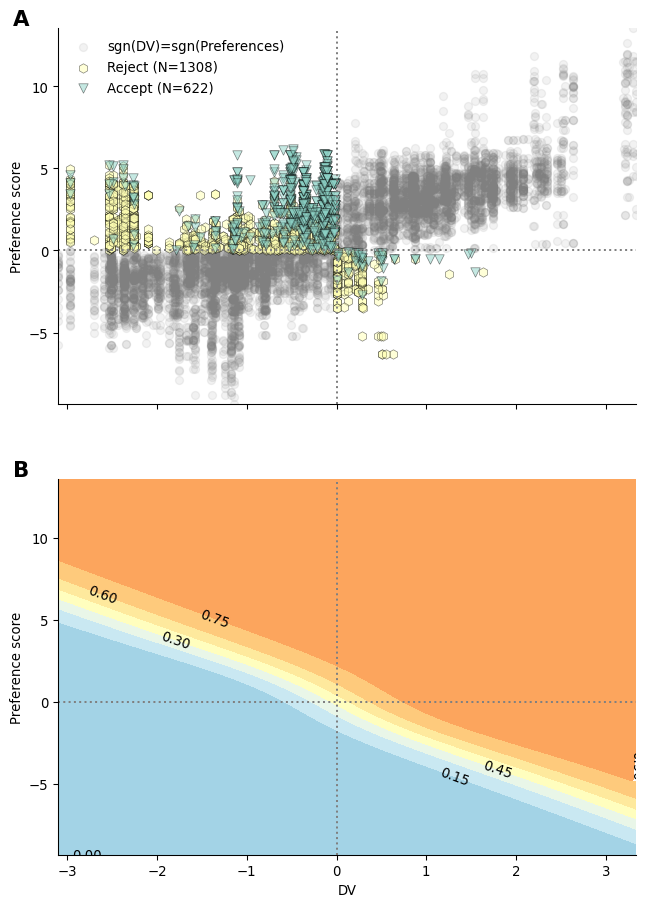
\includegraphics[keepaspectratio]{index_files/figure-latex/S1-supplementary_figures_tables-suppfig-pref-planning-interaction-output-1.png}}

}

\caption{\label{suppfig-pref-planning-interaction}Interaction between
preferences and DV. (A) Participants responses as a function of decision
values of preference score. The response in the off-diagonal quadrants
(top left and bottom right) are color coded per response given, to
highlight that participants responses reflect the strongest signal (tend
to accept despite DV being negative if preferences are high enough). (B)
Fitted probability of accepting as a function of DV and preference
score. Contours with annotations represent a probability of accepting.
The shape of the contour lines highlight that participants choices
reflect the modulation of DV by preference score. The contour trace
indicate that when preference and DV are opposed, participants follow
the strongest signal.}

\end{suppfig}%

\subsection{Supplementary tables:}\label{supplementary-tables}

\begin{supptbl}

\caption{\label{supptbl-model_comparison}}

\centering{

\begin{longtable}[]{@{}
  >{\raggedright\arraybackslash}p{(\linewidth - 10\tabcolsep) * \real{0.2429}}
  >{\raggedleft\arraybackslash}p{(\linewidth - 10\tabcolsep) * \real{0.1714}}
  >{\raggedleft\arraybackslash}p{(\linewidth - 10\tabcolsep) * \real{0.1429}}
  >{\raggedleft\arraybackslash}p{(\linewidth - 10\tabcolsep) * \real{0.1857}}
  >{\raggedleft\arraybackslash}p{(\linewidth - 10\tabcolsep) * \real{0.1286}}
  >{\raggedleft\arraybackslash}p{(\linewidth - 10\tabcolsep) * \real{0.1286}}@{}}
\caption{Main model comparison, comparing the fit of the preference,
context, frequency and pure planning models}\tabularnewline
\toprule\noalign{}
\begin{minipage}[b]{\linewidth}\raggedright
\end{minipage} & \begin{minipage}[b]{\linewidth}\raggedleft
elpd\_loo
\end{minipage} & \begin{minipage}[b]{\linewidth}\raggedleft
p\_loo
\end{minipage} & \begin{minipage}[b]{\linewidth}\raggedleft
elpd\_diff
\end{minipage} & \begin{minipage}[b]{\linewidth}\raggedleft
se
\end{minipage} & \begin{minipage}[b]{\linewidth}\raggedleft
dse
\end{minipage} \\
\midrule\noalign{}
\endfirsthead
\toprule\noalign{}
\begin{minipage}[b]{\linewidth}\raggedright
\end{minipage} & \begin{minipage}[b]{\linewidth}\raggedleft
elpd\_loo
\end{minipage} & \begin{minipage}[b]{\linewidth}\raggedleft
p\_loo
\end{minipage} & \begin{minipage}[b]{\linewidth}\raggedleft
elpd\_diff
\end{minipage} & \begin{minipage}[b]{\linewidth}\raggedleft
se
\end{minipage} & \begin{minipage}[b]{\linewidth}\raggedleft
dse
\end{minipage} \\
\midrule\noalign{}
\endhead
\bottomrule\noalign{}
\endlastfoot
Preference & -1492.49 & 256.526 & 0 & 48.7651 & 0 \\
Context & -1656.69 & 159.175 & 164.209 & 52.4615 & 19.671 \\
Frequency prior & -2073.38 & 77.0896 & 580.889 & 55.5712 & 35.9363 \\
Planning & -2078.46 & 68.3847 & 585.976 & 55.58 & 36.1456 \\
\end{longtable}

}

\end{supptbl}%

\begin{supptbl}

\caption{\label{supptbl-pref_model_param}}

\centering{

\begin{longtable}[]{@{}lrrrr@{}}
\caption{Summary of the parameters of the preference model. The table
displays the mean and 95\% highest density interval (HDI) for the
population level parameters assopciated with the planning values, the
preference regressors and their interaction.}\tabularnewline
\toprule\noalign{}
& mean & sd & hdi\_2.5\% & hdi\_97.5\% \\
\midrule\noalign{}
\endfirsthead
\toprule\noalign{}
& mean & sd & hdi\_2.5\% & hdi\_97.5\% \\
\midrule\noalign{}
\endhead
\bottomrule\noalign{}
\endlastfoot
\(\beta_{plan}\) & 2.072 & 0.242 & 1.614 & 2.573 \\
\(\beta_{O=1}\) & -2.374 & 0.971 & -4.232 & -0.426 \\
\(\beta_{O=2}\) & -1.625 & 0.938 & -3.535 & 0.092 \\
\(\beta_{O=3}\) & 1.627 & 0.945 & -0.22 & 3.453 \\
\(\beta_{O=4}\) & 2.923 & 0.976 & 1.054 & 4.842 \\
\(\beta_{CC=1}\) & 0.765 & 1.161 & -1.488 & 3.105 \\
\(\beta_{CC=2}\) & -0.127 & 1.165 & -2.482 & 2.144 \\
\(\beta_{FC=1}\) & 0.457 & 1.149 & -1.86 & 2.557 \\
\(\beta_{FC=1}\) & 0.21 & 1.149 & -2.051 & 2.359 \\
\(\beta_{E=0}\) & -4.438 & 0.935 & -6.247 & -2.627 \\
\(\beta_{E=1}\) & -0.48 & 0.781 & -1.994 & 1.076 \\
\(\beta_{E=2}\) & -0.02 & 0.75 & -1.473 & 1.492 \\
\(\beta_{E=3}\) & 0.203 & 0.748 & -1.228 & 1.688 \\
\(\beta_{E=4}\) & 0.3 & 0.758 & -1.186 & 1.799 \\
\(\beta_{E=5}\) & 0.793 & 0.769 & -0.602 & 2.44 \\
\(\beta_{E=6}\) & 4.195 & 0.962 & 2.363 & 6.132 \\
\(\beta_{interaction}\) & 1.306 & 0.508 & 0.258 & 2.256 \\
\end{longtable}

}

\end{supptbl}%

\subsection{Supplementary model
comparison}\label{supplementary-model-comparison}

\subsubsection{Preferences model
comparison:}\label{preferences-model-comparison}

The preference model was observed to fit the data best, showing that
participants behavior reflects the integration of a planning component
together with priors reflecting the structure of the task, shedding
light on the structure of the priors themselves. To further show that
participants priors reflect the whole structure of the task, we modelled
the data removing one experimental factor from the preferences fitting
one at a time and compared to the full model, to show that our results
cannot be explained by the fact that participants's priors do not
reflect a single nor a subset of experimental factors. To further show
that participants reliance on planning is modulated by the strength of
their preferenecs, a model without the modulatory effect was fitted to
highlight the increase in fit associated with the modulatory effect of
preferences entropy on DV. Finally, to show that participants response
is best explained by a combination of planning and preference component,
we also fitted a model with only the preference component omitting the
planning regressor.

\begin{suppfig}

\centering{

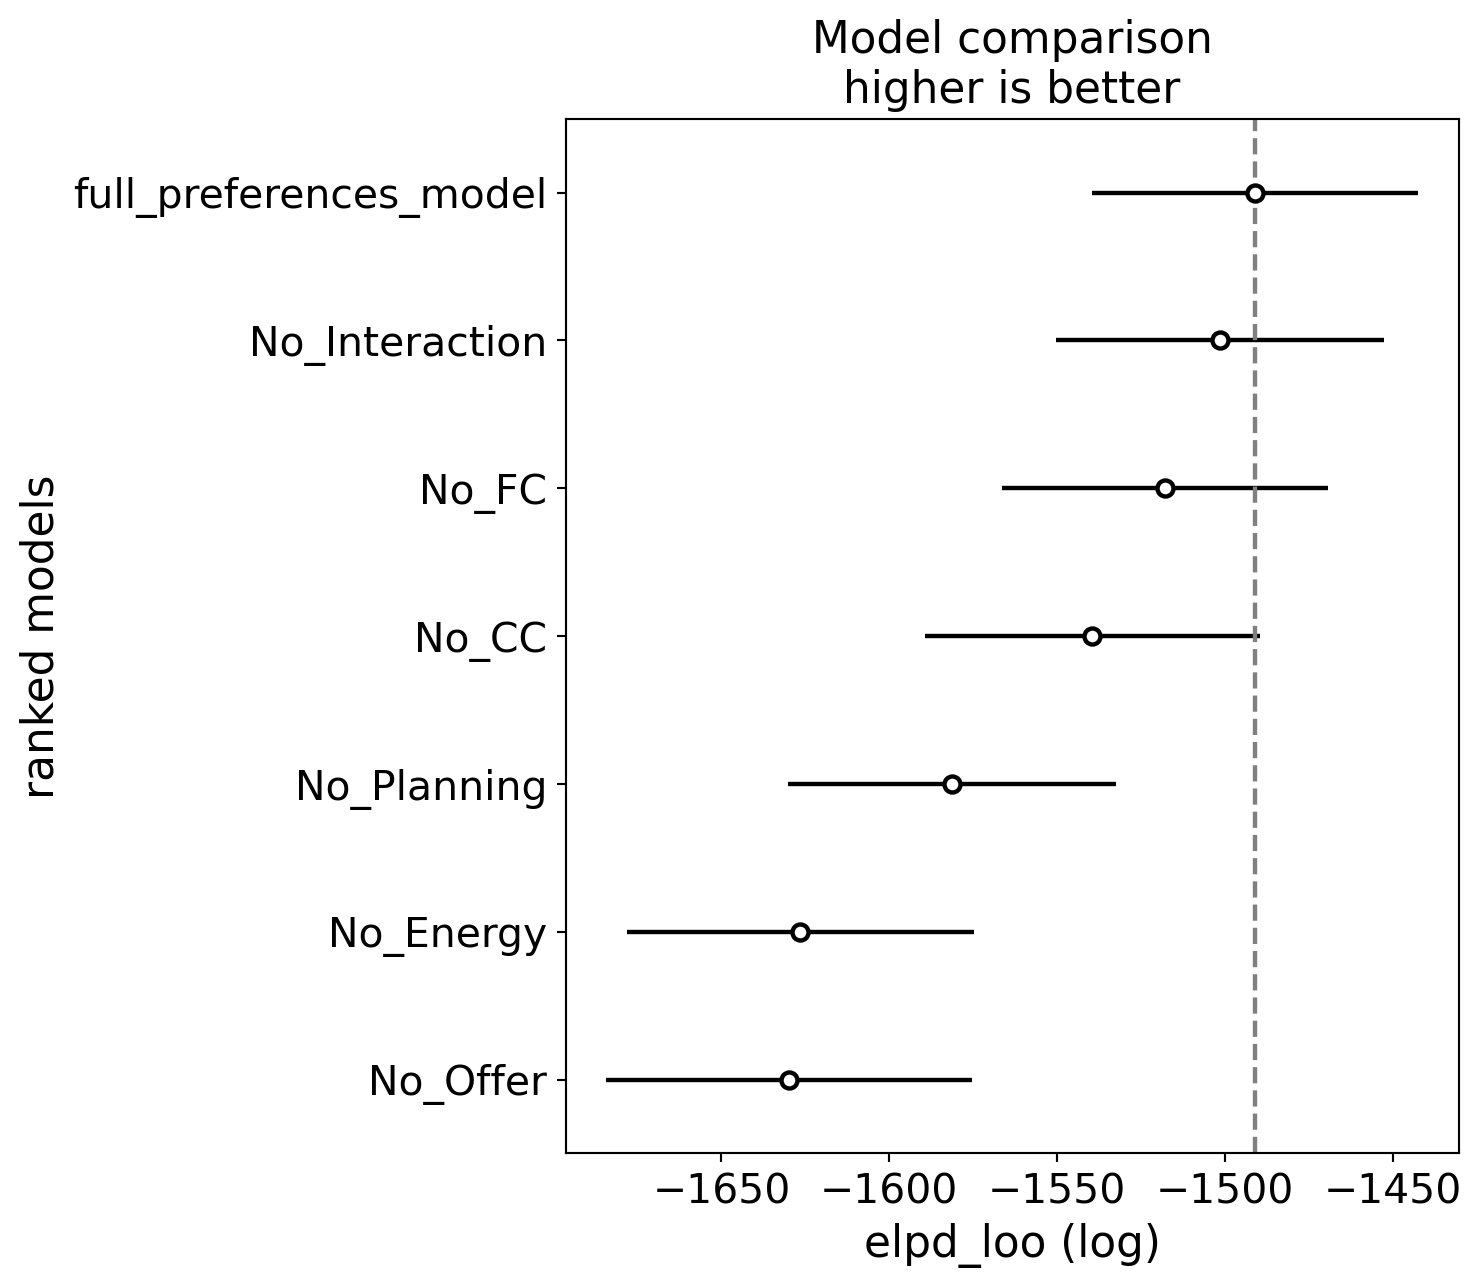
\includegraphics[width=7.72917in,height=6.69792in]{index_files/figure-latex/S2-choice_model_comparison-suppfig-preference_model_comparison-output-1.png}

}

\caption{\label{suppfig-preference_model_comparison}Results of
preferences model comparison. Model abbreviations: (No\_interaction)
model comprising planning and preference component, without interaction
between the two, (No\_FC) model where future cost factor was omitted
from preferences, (No\_CC) model where future cost factor was omitted
from preferences, (No\_Planning) model where DV was omitted,
(No\_Energy) model where energy factor was omitted from preferences,
(No\_Offer) model where offer factor was omitted from preferences}

\end{suppfig}%

\begin{supptbl}

\caption{\label{supptbl-preferences_model_comparison}}

\centering{

\begin{longtable}[]{@{}
  >{\raggedright\arraybackslash}p{(\linewidth - 10\tabcolsep) * \real{0.3117}}
  >{\raggedleft\arraybackslash}p{(\linewidth - 10\tabcolsep) * \real{0.1558}}
  >{\raggedleft\arraybackslash}p{(\linewidth - 10\tabcolsep) * \real{0.1169}}
  >{\raggedleft\arraybackslash}p{(\linewidth - 10\tabcolsep) * \real{0.1688}}
  >{\raggedleft\arraybackslash}p{(\linewidth - 10\tabcolsep) * \real{0.1169}}
  >{\raggedleft\arraybackslash}p{(\linewidth - 10\tabcolsep) * \real{0.1299}}@{}}
\caption{Results of the comparison between different preferences
models}\tabularnewline
\toprule\noalign{}
\begin{minipage}[b]{\linewidth}\raggedright
\end{minipage} & \begin{minipage}[b]{\linewidth}\raggedleft
elpd\_loo
\end{minipage} & \begin{minipage}[b]{\linewidth}\raggedleft
p\_loo
\end{minipage} & \begin{minipage}[b]{\linewidth}\raggedleft
elpd\_diff
\end{minipage} & \begin{minipage}[b]{\linewidth}\raggedleft
se
\end{minipage} & \begin{minipage}[b]{\linewidth}\raggedleft
dse
\end{minipage} \\
\midrule\noalign{}
\endfirsthead
\toprule\noalign{}
\begin{minipage}[b]{\linewidth}\raggedright
\end{minipage} & \begin{minipage}[b]{\linewidth}\raggedleft
elpd\_loo
\end{minipage} & \begin{minipage}[b]{\linewidth}\raggedleft
p\_loo
\end{minipage} & \begin{minipage}[b]{\linewidth}\raggedleft
elpd\_diff
\end{minipage} & \begin{minipage}[b]{\linewidth}\raggedleft
se
\end{minipage} & \begin{minipage}[b]{\linewidth}\raggedleft
dse
\end{minipage} \\
\midrule\noalign{}
\endhead
\bottomrule\noalign{}
\endlastfoot
full\_preferences\_model & -1492.47 & 256.484 & 0 & 48.7583 & 0 \\
No\_Modulation & -1501.44 & 245.861 & 8.9671 & 48.9103 & 5.28966 \\
No\_FC & -1517.79 & 227.725 & 25.3217 & 48.5354 & 7.61146 \\
No\_CC & -1539.49 & 262.803 & 47.0195 & 49.8892 & 9.74314 \\
No\_Planning & -1581.23 & 217.308 & 88.758 & 48.8039 & 17.3434 \\
No\_Energy & -1626.44 & 211.155 & 133.971 & 51.5682 & 17.7893 \\
No\_Offer & -1629.84 & 235.203 & 137.365 & 54.4382 & 19.2265 \\
\end{longtable}

}

\end{supptbl}%

\subsubsection{Frequency model
comparison:}\label{frequency-model-comparison}

In the main text, we compared the preference model with a model in which
priors are computed based on action frequency. In this model, the priors
are computed using a linearly decaying moving average, discounting
actions that occured further in the past. We presented the results
obtained when the priors are derived from the 20 previous trials. This
number of trials was selected by exploring priors witk
\(k=[2, 5, 10, 15, 20, 30, 50]\) to identify the values that fit the
data the best:

\begin{suppfig}

\centering{

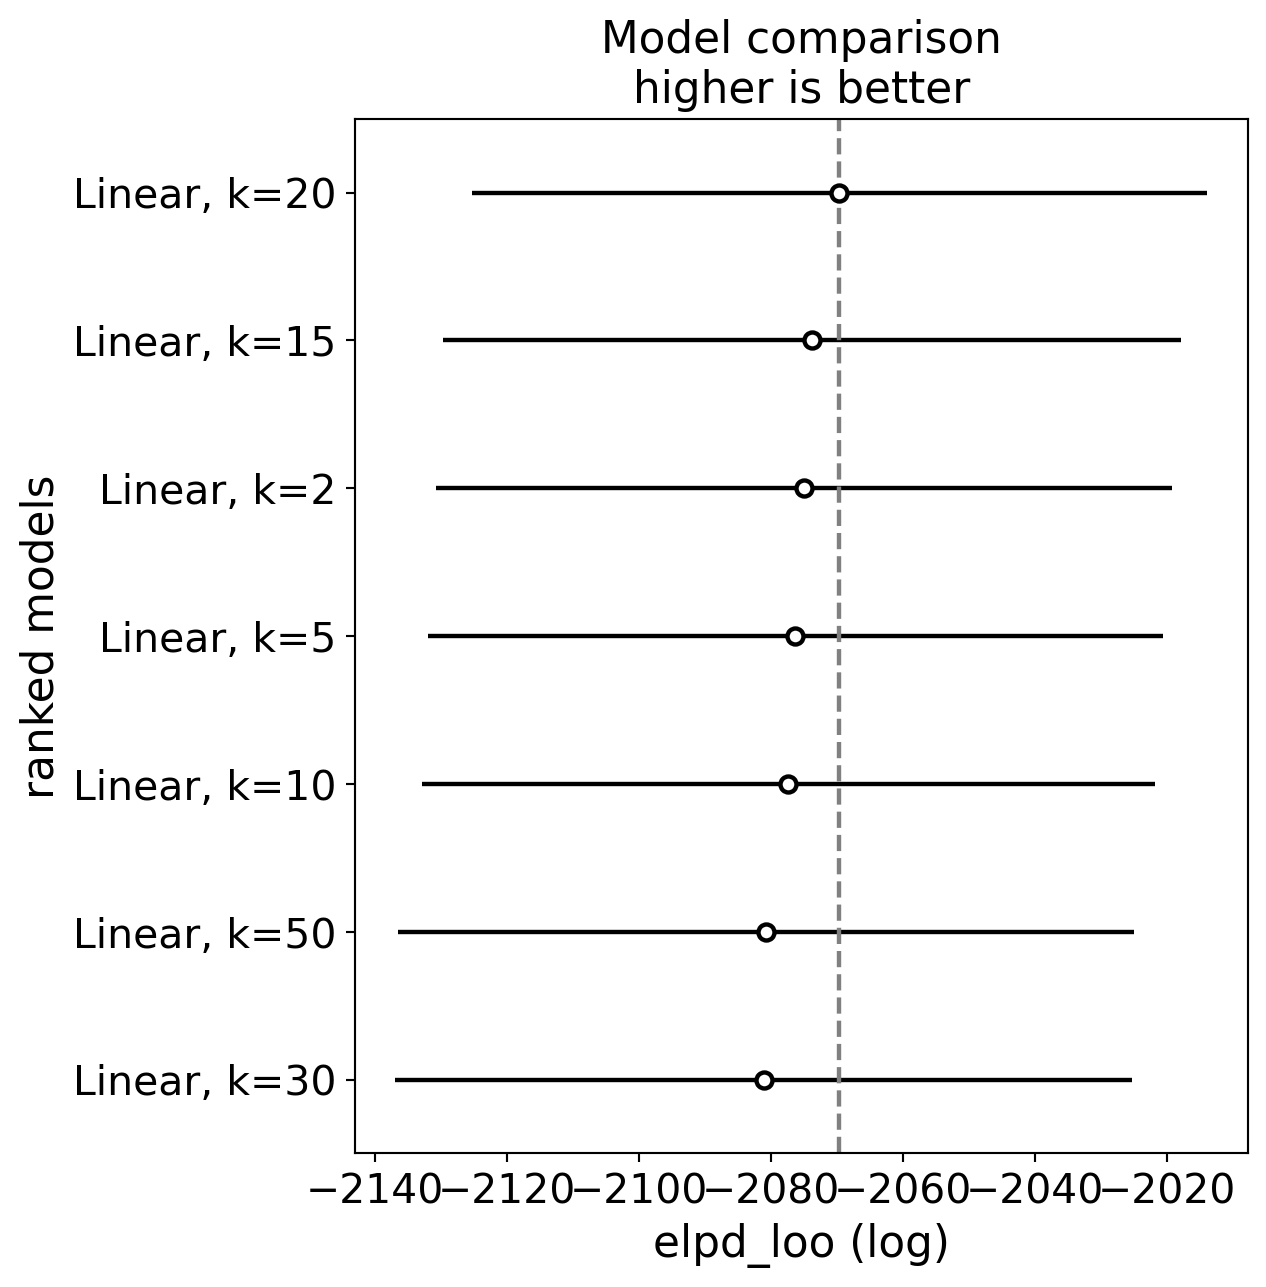
\includegraphics[width=6.59375in,height=6.69792in]{index_files/figure-latex/S2-choice_model_comparison-suppfig-frequency_model_comparison-output-1.png}

}

\caption{\label{suppfig-frequency_model_comparison}Results of frequency
model comparison, comparing the temporal integration window, going back
k={[}2, 5, 10, 15, 20, 30, 50{]}}

\end{suppfig}%

\begin{supptbl}

\caption{\label{supptbl-frequency_model_comparison}}

\centering{

\begin{longtable}[]{@{}
  >{\raggedright\arraybackslash}p{(\linewidth - 10\tabcolsep) * \real{0.2121}}
  >{\raggedleft\arraybackslash}p{(\linewidth - 10\tabcolsep) * \real{0.1818}}
  >{\raggedleft\arraybackslash}p{(\linewidth - 10\tabcolsep) * \real{0.1364}}
  >{\raggedleft\arraybackslash}p{(\linewidth - 10\tabcolsep) * \real{0.1970}}
  >{\raggedleft\arraybackslash}p{(\linewidth - 10\tabcolsep) * \real{0.1364}}
  >{\raggedleft\arraybackslash}p{(\linewidth - 10\tabcolsep) * \real{0.1364}}@{}}
\caption{Results of the frequency model comparisons with different
temporal integration windows}\tabularnewline
\toprule\noalign{}
\begin{minipage}[b]{\linewidth}\raggedright
\end{minipage} & \begin{minipage}[b]{\linewidth}\raggedleft
elpd\_loo
\end{minipage} & \begin{minipage}[b]{\linewidth}\raggedleft
p\_loo
\end{minipage} & \begin{minipage}[b]{\linewidth}\raggedleft
elpd\_diff
\end{minipage} & \begin{minipage}[b]{\linewidth}\raggedleft
se
\end{minipage} & \begin{minipage}[b]{\linewidth}\raggedleft
dse
\end{minipage} \\
\midrule\noalign{}
\endfirsthead
\toprule\noalign{}
\begin{minipage}[b]{\linewidth}\raggedright
\end{minipage} & \begin{minipage}[b]{\linewidth}\raggedleft
elpd\_loo
\end{minipage} & \begin{minipage}[b]{\linewidth}\raggedleft
p\_loo
\end{minipage} & \begin{minipage}[b]{\linewidth}\raggedleft
elpd\_diff
\end{minipage} & \begin{minipage}[b]{\linewidth}\raggedleft
se
\end{minipage} & \begin{minipage}[b]{\linewidth}\raggedleft
dse
\end{minipage} \\
\midrule\noalign{}
\endhead
\bottomrule\noalign{}
\endlastfoot
Linear, k=20 & -2069.6 & 78.3873 & 0 & 55.6858 & 0 \\
Linear, k=15 & -2073.74 & 74.2703 & 4.13799 & 55.8878 & 5.24083 \\
Linear, k=2 & -2074.98 & 75.5677 & 5.37448 & 55.6833 & 6.29665 \\
Linear, k=5 & -2076.3 & 78.84 & 6.69933 & 55.6484 & 5.58139 \\
Linear, k=10 & -2077.34 & 74.0643 & 7.73213 & 55.5341 & 5.65329 \\
Linear, k=50 & -2080.71 & 78.7902 & 11.1052 & 55.7161 & 5.09526 \\
Linear, k=30 & -2081.1 & 75.786 & 11.4922 & 55.7602 & 5.46973 \\
\end{longtable}

}

\end{supptbl}%

\subsection{Parameters recovery:}\label{parameters-recovery}

In the main text, the preference model was observed to fit participants
behavior the best, supporting the hypothesis that participants decision
reflects the integration of forward planning with state dependent
preferences. The preferences model is rather complex, with preference
parameters being estimated as latent variable, and entailing an
additional entropy transformation in the interaction term. To establish
that despite the complexity of the model, it is still capable of
accurately estimate all parameters, we perform a parameter recovery
analysis in which we simulate data using the mean parameters recovered
from the original data. We then fit the same model to the simulated
data. We can then compare the estimated parameters from the simulated
data against ground truth to establish the model capacity to identify
parameters correctly.

\begin{suppfig}

\centering{

\pandocbounded{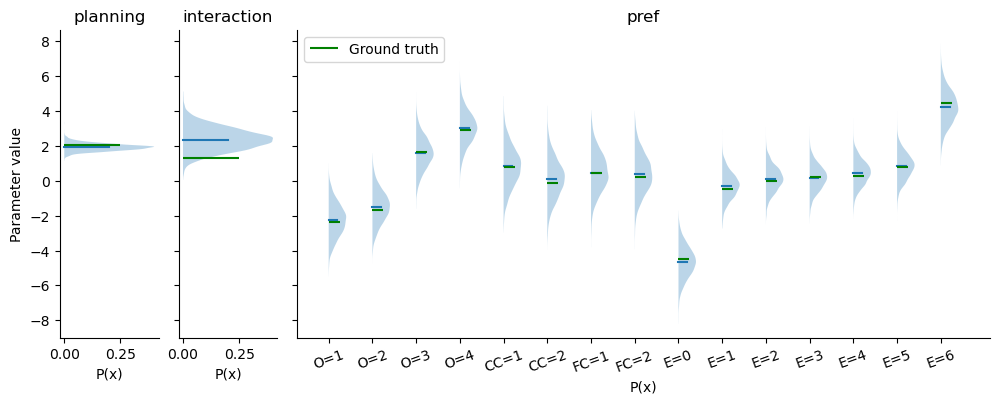
\includegraphics[keepaspectratio]{index_files/figure-latex/S3-parameters_recovery-suppfig-population_parameter_recovery-output-1.png}}

}

\caption{\label{suppfig-population_parameter_recovery}Population level
parameters recovery}

\end{suppfig}%

Across all participants, the ground truth parameters is well within the
credible intervals of the retrieved parameters from the data, indicating
that our model is indeed capable of recovering the parameters of the
underlying generative model.




\end{document}
